% This is the Reed College LaTeX thesis template. Most of the work
% for the document class was done by Sam Noble (SN), as well as this
% template. Later comments etc. by Ben Salzberg (BTS). Additional
% restructuring and APA support by Jess Youngberg (JY).
% Your comments and suggestions are more than welcome; please email
% them to cus@reed.edu
%
% See https://www.reed.edu/cis/help/LaTeX/index.html for help. There are a
% great bunch of help pages there, with notes on
% getting started, bibtex, etc. Go there and read it if you're not
% already familiar with LaTeX.
%
% Any line that starts with a percent symbol is a comment.
% They won't show up in the document, and are useful for notes
% to yourself and explaining commands.
% Commenting also removes a line from the document;
% very handy for troubleshooting problems. -BTS

% As far as I know, this follows the requirements laid out in
% the 2002-2003 Senior Handbook. Ask a librarian to check the
% document before binding. -SN

%%
  %% Preamble
%%
  % \documentclass{<something>} must begin each LaTeX document
\documentclass[12pt,twoside]{smiththesis}
% Packages are extensions to the basic LaTeX functions. Whatever you
% want to typeset, there is probably a package out there for it.
% Chemistry (chemtex), screenplays, you name it.
% Check out CTAN to see: https://www.ctan.org/
  %%
  \usepackage{graphicx,latexsym}
\usepackage{amsmath}
\usepackage{amssymb,amsthm}
\usepackage{longtable,booktabs,setspace}
\usepackage{chemarr} %% Useful for one reaction arrow, useless if you're not a chem major
\usepackage[hyphens]{url}
% Added by CII
\usepackage{hyperref}
\usepackage{lmodern}
\usepackage{multicol}
\usepackage{float}
\floatplacement{figure}{H}
% End of CII addition
\usepackage{rotating}
%\hypersetup{
%    colorlinks=true,
%    linkcolor=blue,
%    filecolor=magenta,      
 %   urlcolor=blue,
 %   pdftitle={Overleaf Example},
 %   pdfpagemode=FullScreen,
 %   }

% Next line commented out by CII
%%% \usepackage{natbib}
% Comment out the natbib line above and uncomment the following two lines to use the new
% biblatex-chicago style, for Chicago A. Also make some changes at the end where the
% bibliography is included.
%\usepackage{biblatex-chicago}
%\bibliography{thesis}


% Added by CII (Thanks, Hadley!)
% Use ref for internal links
\renewcommand{\hyperref}[2][???]{\autoref{#1}}
\def\chapterautorefname{Chapter}
\def\sectionautorefname{Section}
\def\subsectionautorefname{Subsection}
% \hypersetup{
%     colorlinks=true,
%     linkcolor=blue,
%    filecolor=blue,
%     citecolor = blue,      
%     urlcolor=cyan,
 %    }
\hypersetup{colorlinks=true,
            linkcolor=blue,
            citecolor=black,
            urlcolor=blue}
% End of CII addition

% Added by CII
\usepackage{caption}
\captionsetup{width=5in}
% End of CII addition

% \usepackage{times} % other fonts are available like times, bookman, charter, palatino
\usepackage{palatino}
\usepackage{tcolorbox}

% Syntax highlighting #22

% To pass between YAML and LaTeX the dollar signs are added by CII
\title{Estimating Unobserved COVID-19 Infections in the United States}
\author{Quinn White}
% The month and year that you submit your FINAL draft TO THE LIBRARY (May or December)
\date{May 2023}
\division{Mathematics and Natural Sciences}
\advisor{Ben Baumer}
\institution{Smith College}
\degree{Bachelor of Arts}
%If you have two advisors for some reason, you can use the following
% Uncommented out by CII
\altadvisor{Nicholas Reich}
% End of CII addition

%%% Remember to use the correct department!
\department{Statistical and Data Sciences}
% if you're writing a thesis in an interdisciplinary major,
% uncomment the line below and change the text as appropriate.
% check the Senior Handbook if unsure.
%\thedivisionof{The Established Interdisciplinary Committee for}
% if you want the approval page to say "Approved for the Committee",
% uncomment the next line
%\approvedforthe{Committee}

% Added by CII
%%% Copied from knitr
%% maxwidth is the original width if it's less than linewidth
%% otherwise use linewidth (to make sure the graphics do not exceed the margin)
\makeatletter
\def\maxwidth{ %
  \ifdim\Gin@nat@width>\linewidth
    \linewidth
  \else
    \Gin@nat@width
  \fi
}
\makeatother

\newlength{\csllabelwidth}
\setlength{\csllabelwidth}{3em}
\newlength{\cslhangindent}
\setlength{\cslhangindent}{1.5em}
% for Pandoc 2.8 to 2.10.1
\newenvironment{cslreferences}%
  {}%
  {\par}
% For Pandoc 2.11+
% As noted by @mirh [2] is needed instead of [3] for 2.12
\newenvironment{CSLReferences}[2] % #1 hanging-ident, #2 entry spacing
 {% don't indent paragraphs
\setlength{\parindent}{0pt}
% turn on hanging indent if param 1 is 1
\ifodd #1 \everypar{\setlength{\hangindent}{\cslhangindent}}\ignorespaces\fi
% set entry spacing
\ifnum #2 > 0
\setlength{\parskip}{#2\baselineskip}
  \fi
}%
{}
\usepackage{calc} % for calculating minipage widths
\newcommand{\CSLBlock}[1]{#1\hfill\break}
  \newcommand{\CSLLeftMargin}[1]{\parbox[t]{\csllabelwidth}{#1}}
    \newcommand{\CSLRightInline}[1]{\parbox[t]{\linewidth - \csllabelwidth}{#1}}
      \newcommand{\CSLIndent}[1]{\hspace{\cslhangindent}#1}
        \renewcommand{\contentsname}{Table of Contents}
% End of CII addition

\setlength{\parskip}{0pt}

% Added by CII

\providecommand{\tightlist}{%
  \setlength{\itemsep}{0pt}\setlength{\parskip}{0pt}}

\Acknowledgements{
Will add
}

\Dedication{
You can have a dedication here if you wish.
}


\Abstract{
As we have navigated the COVID-19 pandemic, case counts have been a central source of information for understanding transmission dynamics and the effect of public health interventions. However, because the number of cases we observe is limited by the testing effort in a given location, the case counts presented on local or national dashboards are only a fraction of the true infections. Variations in testing rate by time and location impacts the number of cases that go unobserved, which can cloud our understanding of the true COVID-19 incidence at a given time point and can create biases in downstream analyses. Additionally, the number of cases we observe is impacted by the sensitivity and specificity of the diagnostic test. To quantify the number of true infections given incomplete testing and diagnostic test inaccuracy, this work implements probabilistic bias analysis at a biweekly time scale from January 1, 2021 through February 2022. In doing so, we can estimate a range of possible true infections for a given time interval and location. This approach can be applied at the state level across the United States, as well as in some counties where the needed data are available.
}

	\usepackage{booktabs}
\usepackage{longtable}
\usepackage{array}
\usepackage{multirow}
\usepackage{wrapfig}
\usepackage{float}
\usepackage{colortbl}
\usepackage{pdflscape}
\usepackage{tabu}
\usepackage{threeparttable}
\usepackage{threeparttablex}
\usepackage[normalem]{ulem}
\usepackage{makecell}
\usepackage{xcolor}
% End of CII addition
%%
%% End Preamble
%%
%
\begin{document}

% Everything below added by CII
  \maketitle

\frontmatter % this stuff will be roman-numbered
\pagestyle{empty} % this removes page numbers from the frontmatter
  \begin{acknowledgements}
    Will add
  \end{acknowledgements}

% https://github.com/ismayc/thesisdown/issues/32 
  {
    \hypersetup{linkcolor=black}
    \setcounter{tocdepth}{2}
    \tableofcontents
  }


  \begin{abstract}
    As we have navigated the COVID-19 pandemic, case counts have been a central source of information for understanding transmission dynamics and the effect of public health interventions. However, because the number of cases we observe is limited by the testing effort in a given location, the case counts presented on local or national dashboards are only a fraction of the true infections. Variations in testing rate by time and location impacts the number of cases that go unobserved, which can cloud our understanding of the true COVID-19 incidence at a given time point and can create biases in downstream analyses. Additionally, the number of cases we observe is impacted by the sensitivity and specificity of the diagnostic test. To quantify the number of true infections given incomplete testing and diagnostic test inaccuracy, this work implements probabilistic bias analysis at a biweekly time scale from January 1, 2021 through February 2022. In doing so, we can estimate a range of possible true infections for a given time interval and location. This approach can be applied at the state level across the United States, as well as in some counties where the needed data are available.
  \end{abstract}
  \begin{dedication}
    You can have a dedication here if you wish.
  \end{dedication}
\mainmatter % here the regular arabic numbering starts
\pagestyle{fancyplain} % turns page numbering back on

\hypertarget{motivation}{%
\chapter{Motivation}\label{motivation}}

Placeholder

\hypertarget{background}{%
\chapter{Background}\label{background}}

\hypertarget{probabalistic-bias-analysis}{%
\section{Probabalistic Bias Analysis}\label{probabalistic-bias-analysis}}

Often the focus of quantifying error about an effect estimate focuses on random error rather than the systematic error. For example, typical frequentist confidence intervals are frequent in medical and epidemiological literature, although they have faced rising criticism (Greenland et al., 2016). These confidence intervals quantify the fraction of the times we expect the true value to fall in this interval under the assumption that our model is correct. That is, if we ran an experiment 100 times and computed the effect size each time, we would expect the 95\% confidence interval to contain the true value to 95 of those times, on average. Neyman stressed this in his original publication formalizing the concept of a confidence interval in 1937 (Neyman, 1937). The nuance that the confidence interval is not the probability that the true value falls within this interval, however, is often lost in the discussion of results, in part because the true meaning of a confidence interval is less intuitive.

The aim of quantitative bias analysis is to estimate systematic error to give a range of possible values for the true quantity of interest. In this sense, it is a type of sensitivity analysis. It can be used to estimate various kinds of biases, from misclassification, as is implemented in this work, as well as selection bias and unmeasured confounding (Petersen, Ranker, Barnard-Mayers, MacLehose, \& Fox, 2021). Often, the goal of performing such an analysis is to see how these sources of bias affect our estimates; in particular, under what situations of bias the observed effect would be null.

There are multiple different forms of bias analysis (Lash, Fox, \& Fink, 2009). The most simple case, simple bias analysis, is correcting a point estimate for a single source of error. Multidimensional bias analysis extends this to consider sets of bias parameters, but still provides a corrected point estimate rather than a range of plausible estimates. Probabilistic bias analysis, meanwhile, defines probability distributions for bias parameters to generate a distribution of corrected estimates by repeatedly correcting estimates for bias under different combinations of the parameter values. Then, via Monte Carlo we obtain a distribution of corrected estimates that reflect the corrected values under different scenarios of bias, that is, under different combinations of the bias parameters. This can give us a better idea for the extent of uncertainty about the corrected estimates, although this uncertainty does depend on the specification of the bias parameter distributions. Inherent in bias analysis is the dependence of our results on the specification of bias parameters, which reflect what is known from available data, literature, or theory on the extent of bias that may occur. There is uncertainty about how we define these distributions or values; otherwise, if the precise values of the bias parameters were known, we could simply correct the estimates and probabilistic bias analysis would not be useful.

Although some forms of probabilistic bias analysis can be applied to summarized data, for example, frequencies in a contingency table, the methods are most often implemented with unsummarized data in its original form, as implemented here.

In choosing specific distributions for the bias parameters, different specifications may yield density functions where most of the density is within a similar interval, which means the choice of the specific distribution will not be sensitive to the particular choice of density.

\hypertarget{background-for-the-approach}{%
\section{Background for the Approach}\label{background-for-the-approach}}

The Bayesian melding approach was proposed by Poole et al. (Poole \& Raftery, 2000).

This approach enables us to account for both uncertainty from inputs and outputs of a deterministic model. The initial motivation for the approach was to study the population dynamics of whales in the presence of substantial uncertainty around model inputs for population growth (Poole \& Raftery, 2000). However, the framework provided by Poole et al.~can applied in any circumstance where we have uncertainty around some quantities \(\theta\) and \(\phi\) where there is a deterministic function \(M:\theta \to\phi\). Due the utility of Bayesian melding in various contexts, since this deterministic model \(M\) could take on a wide range of forms, the approach has since been applied in various fields, including urban simulations (Ševčíková, Raftery, \& Waddell, 2007), ecology (Robson, 2014), and infectious disease (Powers et al., 2011).

Let \(M: \theta \to \phi\) be the deterministic model defined by the function relating a vector of input parameters \(\theta\) to an output vector \(\phi\), and suppose we have a prior on \(\theta\) denoted \(f_\theta(\theta)\) and a prior on \(\phi\) denoted \(f_\phi^{direct}(\phi)\).

However, note that we actually have two distinct priors on \(\phi\). There is the prior formed by the distribution induced on \(\phi\) by the prior for \(\theta\) and the function \(M\), where we denote this induced prior \(f_\phi^{induced}(\phi)\). Generally, these priors are based on different sources of information.

If \(M^{-1}\) exists, we can write this induced prior \(f_\phi^{induced}(\phi) = f_\theta(M^{-1}(\phi)) |J(\phi)|\)\footnote{In the continuous case we need to multiply by \(|J(\phi)|\), but not in the discrete case (Blitzstein \& Hwang, 2019).}. This result follows from the fact \(M(\theta) = \phi\), so we apply a change of variables to obtain the distribution of \(\phi\) from the distribution of \(M(\theta)\).

In practice, \(M^{-1}\) rarely exists exists since \(\theta\) is often of higher dimensionality then \(\phi\), in which cases \(M\) is not invertible. This means we generally approximate \(f_\phi^{induced}\) without acquiring its analytical form.

In addition to this induced prior, we have the prior \(f_\phi^{direct}(\phi)\), which does not involve \(M\) nor the inputs \(\theta\). Since these priors are based on different sources of information and may reflect different uncertainties, often it useful to use both sources of information to inform our estimates. To do so, we need to combine the distributions for \(f_\phi^{induced}\) and \(f_\phi^{direct}\) to create a pooled distribution.

Multiple pooling strategies exist for distinct distributions, but one requirement for a Bayesian analysis is that the distribution should be independent of the order in which the prior is updated and the combining of the prior distribution. That is, updating the prior distributions using Bayes' theorem and then combining distributions should yield the same result as combining distributions and then updating this combined distribution; pooling methods that have this property are deemed externally Bayesian. Logarithmic pooling has been shown to be externally Bayesian under some conditions, which are likely to hold in most settings. Furthermore, logarithmic pooling has actually been shown to be the only pooling method where this holds (Genest, McConway, \& Schervish, 1986). For this reason, Poole \emph{et al.} recommend proceeding with logarithmic pooling for Bayesian melding.

The logarithmically pooled prior for \(\phi\) by pooling \(f_\phi^{induced}\) and \(f_\phi^{direct}\) is

\[f_\phi^{pooled} (\phi) = t(\boldsymbol{\alpha}) (f_\phi^{induced}(\phi))^{\alpha} (f_\phi^{direct}(\phi))^{1-\alpha}\]

where \(\alpha \in [0,1]\) is a pooling weight and \(t(\boldsymbol{\alpha})\) is the normalizing constant. Commonly, a choice of \(\alpha = 0.5\) is used to give the priors equal weight. In this case, logarithmic pooling may be referred to as geometric pooling since it is equivalent to taking a geometric mean.

If \(M\) is invertible, we can obtain the contrained distributions for the model inputs by simply inverting \(M\). However, \(M\) is rarely invertible, so we have to think about how to proceed in the noninvertible case.

\hypertarget{simple-discrete-example}{%
\subsection{Simple Discrete Example}\label{simple-discrete-example}}

To get intuition for a valid strategy Poole et al.~recommend, we consider a mapping \(M: \theta \to \phi\) for \(\theta \in \mathbb{R}\) and \(\phi \in \mathbb{R}\)
defined as follows (Figure \ref{fig:dex}). Note the choice of \(f_\theta,f_\phi^{direct}\) does not matter here as long as they are valid densities.
\begin{multicols}{2}
\begin{figure}

{\centering 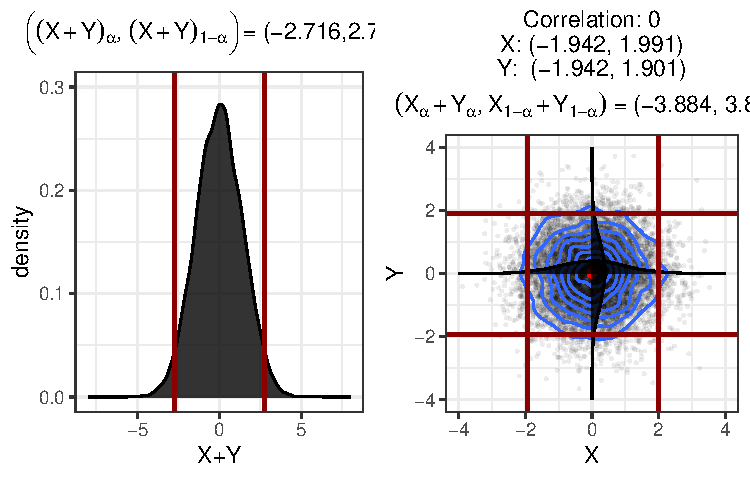
\includegraphics{thesis_files/figure-latex/unnamed-chunk-4-1} 

}

\caption{\label{fig:dex}A simple discrete example where $M$ is not invertible.}\label{fig:unnamed-chunk-4}
\end{figure}
\columnbreak
\begin{table}[H]
\centering
\begin{tabular}[t]{r|r|r|r}
\hline
$\theta$ & $f_\theta(\theta)$ & $M(\theta)=\phi$ & $f_\phi^{direct}(\phi)$\\
\hline
1 & 0.3 & 1 & 0.4\\
\hline
2 & 0.2 & 2 & 0.6\\
\hline
3 & 0.5 & 2 & 0.6\\
\hline
\end{tabular}
\end{table}
\end{multicols}
We see that \(M\) is not invertible since \(\theta=1\) and \(\theta = 2\) both map to \(\phi=2\), which implies the inverse \(M^{-1}\) would not be well defined.

We can generate a sample from the density \(f_\phi^{induced}\) by sampling from \(f_\theta\) and computing \(M(\theta)\).

So we have
\begin{align*}
f_\phi^{induced}(1) &= f_{\theta}(1) = 0.3 & \text{ (since $\theta = 1$ maps $\phi = 1$) } \\
f_\phi^{induced}(2) &= f_{\theta}(2) +  f_{\theta}(3) = 0.2 + 0.5=  0.7 & \text{ (since $\theta = 2$ and $\theta=3$ both map to $\phi = 2$) }
\end{align*}
Then, we can compute the logarithmically pooled pooled prior with \(\alpha=0.5\) by taking \(f_\phi^{induced}(\phi)^{\alpha} f_\phi^{direct}(\phi)^{1-\alpha}\).

This gives us
\begin{align*}
f_\phi^{induced}(\phi)^{\alpha} f_\phi^{direct}(\phi)^{1-\alpha} &= (0.3)^{0.5}(0.4)^{0.5} = 0.3464\\
f_\phi^{induced}(\phi)^{\alpha} f_\phi^{direct}(\phi)^{1-\alpha} &= (0.7)^{0.5}(0.6)^{0.5} = 0.6481.
\end{align*}
To make this a valid density, however, these probabilities must sum to 1, so we renormalize by dividing by (0.3464 + 0.6481). Denoting the pooled prior in phi-space as \(f_\phi^{pooled}(\phi)\), this gives us
\begin{align*}
f_\phi^{pooled}(1) &= \frac{ 0.3464  }  { 0.3464 + 0.6481 } = 0.3483 \\
f_\phi^{pooled}(2) &= \dfrac{ 0.6481 } { 0.3464 + 0.6481}  =0.6517.
\end{align*}
We summarize these results and compare \(f_\phi^{induced}, f_\phi^{direct}\), and \(f_\phi^{pooled}\) in Figure \ref{fig:comp}.
\begin{multicols}{2}
\begin{table}[H]
\centering
\begin{tabular}[t]{r|r|r|r}
\hline
$\phi$ & $f_\phi^{direct}(\phi)$ & $f_\phi^{induced}(\phi)$ & $f_\phi^{pooled}(\phi)$\\
\hline
1 & 0.4 & 0.3 & 0.3483\\
\hline
2 & 0.6 & 0.7 & 0.6517\\
\hline
\end{tabular}
\end{table}
\columnbreak
\begin{figure}

{\centering 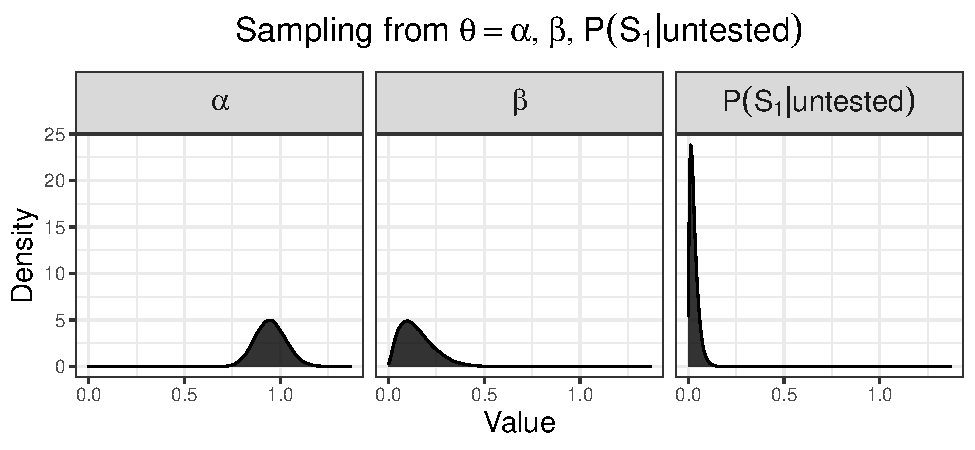
\includegraphics{thesis_files/figure-latex/unnamed-chunk-7-1} 

}

\caption{\label{fig:comp}}\label{fig:unnamed-chunk-7}
\end{figure}
\end{multicols}
However, we also want the pooled prior on the inputs \(\theta\), that is, \(f_\theta^{pooled}(\theta)\).

Poole et al.~reasoned as follows. Since \(M\) uniquely maps \(\theta=1\) to \(\phi =1\), the probability that \(\theta=1\) should be equal to the probability \(\phi = 1\). That is, we should have \(f_\theta^{pooled}(1) = f_\phi^{pooled}(1)\).

However, the relationship for \(\theta=2\) or \(\theta=3\) to \(\phi\) is not one to one. Since \(M(2)=2\) and \(M(3)=2\), the sum of the probabilities for \(\theta=1\) and \(\theta=2\) should be equal to that for \(\phi=2\), that is, \(f_\theta^{pooled}(2) + f_\theta^{pooled}(3) = f_\phi^{pooled}(2) = 0.6517\).

The challenge here is how we divide the probability for \(f_\phi^{pooled}(2)\), which is defined, among \(f_\theta^{pooled}(2)\) and \(f_\theta^{pooled}(3)\). The prior for \(\phi\) yields no information to assist in this choice, because knowing which value \(\phi\) takes on does not give us any information about whether \(\theta=2\) or \(\theta=3\). Thus, the information we have about \(\theta\) must be taken from \(f_\theta(\theta)\).

That is, we can assign a probability for \(f_\theta^{pooled}(2)\) by considering the probability that \(\theta = 2\) relative to the probability \(\theta =3\), computing

\[f_\theta^{pooled}(2) = f_\phi^{pooled}(2) \Big( \frac{f_\theta(2)}{f_\theta(2) + f_\theta(3)}\Big).\]

That is, if the probability \(\theta\) takes on the value \(2\) is lower in this case than the probability \(\theta=3\) which we know from the prior on \(\theta\), \(f_\theta(\theta)\), then the pooled prior on \(\theta\), \(f_\theta^{pooled}(2)\), should reflect this.

Using this reasoning, we have
\begin{align*} f_\theta^{pooled}(2) &= (0.7) \frac{0.2}{0.2+0.5} = 0.1862\\
f_\theta^{pooled}(3) &= (0.7) \frac{0.5}{0.2+0.5} = 0.4655.
\end{align*}
The result in this simple example, using \(f_\theta(\theta)\) to determine how to distribute the probability for values of \(\phi\) where multiple \(\theta\) map to \(\phi\), can be used to derive general formulas to compute \(f_\theta^{pooled}(\theta)\) for discrete and continuous distributions (Poole \& Raftery, 2000).

\hypertarget{general-solution-for-the-discrete-case}{%
\subsection{General Solution for the Discrete Case}\label{general-solution-for-the-discrete-case}}

Denote the possible values of \(\theta\) as \(A_1, A_2, \dots\), the possible values of \(\phi\) as \(B_1, B_2, \dots\), and a mapping \(m: \mathbb{N} \to \mathbb{N}\) such that \(M(A_i) = B_{m(i)}\) and \(C_j = M^{-1}(B_j) = \{A_i : M(A_i) = B_j\}\). Then

\[f_\theta^{pooled}(A_i) = f_\phi^{pooled}(B_{m(i)}) \left( \frac{f_\theta(A_i)}{f_\phi^{induced}(B_{m(i)})} \right).\]

\hypertarget{general-solution-for-the-continuous-case}{%
\subsection{General Solution for the Continuous Case}\label{general-solution-for-the-continuous-case}}

We denote \(B = M(A) = \{M(\theta) : \theta \in A \}\) and \(C = M^{-1}(B) = \{\theta: M(\theta) \in B \}\).

Then

\[
f_\phi^{pooled} (M(\theta)) =t({\alpha}) f_\theta(\theta) \left( \frac{f_\phi^{direct}(M(\theta))}{f_\phi^{induced}(M(\theta))} \right)^{1-\alpha} \tag{2}
\]
where \(t({\alpha})\) is a renormalizing constant for the choice of \(\alpha\).

\hypertarget{implementation-through-the-sampling-importance-resampling-algorithm}{%
\subsection{Implementation through the Sampling-Importance-Resampling Algorithm}\label{implementation-through-the-sampling-importance-resampling-algorithm}}

We can obtain the pooled distributions \(f^{pooled}_\theta\) and \(f^{pooled}_\phi\) by using the Sampling-Importance-Resampling Algorithm.

The steps are as follows.
\begin{enumerate}
\def\labelenumi{\arabic{enumi}.}
\tightlist
\item
  We draw \(\theta\) from its prior distribution \(f_\theta(\theta)\).
\item
  For every \(\theta_i\) we compute \(\phi_i = M(\theta_i)\) to obtain a sample from the induced distribution.
\item
  Since the density \(f_\phi^{induced}(\phi)\) is unlikely to have an analytical form, we can compute it via a density approximation such as kernel density estimation.
\item
  Construct weights proportional to the ratio of the prior on \(\phi\) evaluated at \(M(\theta_i)\) to the induced prior \(f_\phi^{induced}\) evaluated at \(M(\theta_i)\). If a likelihood \(L_1(\theta)\) for the inputs and \(L_2(\phi)\) is available, the weights are
  \[w_i = \left( \frac{f_\phi^{direct}(M(\theta_i))}{f_\phi^{induced}(M(\theta_i))} \right)^{1-\alpha}.\]
  However, in this work, no likelihood is available for the variables of interest, so the likelihood is left out of the weights, leaving us with
  \[w_i = \left( \frac{f_\phi^{direct}(M(\theta_i))}{f_\phi^{induced}(M(\theta_i))} \right)^{1-\alpha}.\]
\item
  Sample \(\theta\) and \(\phi\) from step (1) with probabilities proportional to the weights from (4).
\end{enumerate}
\newpage

\hypertarget{bayesian-melding-applied-to-covid-19-misclassification}{%
\section{Bayesian Melding Applied to COVID-19 Misclassification}\label{bayesian-melding-applied-to-covid-19-misclassification}}

~~~In this work, we can relate the inputs \(\theta = \{P(S_1|\text{untested}), \alpha, \beta \}\) and \(\phi = P(S_0|\text{test}_+,\text{untested})\) by the deterministic model \(M: \theta \to \phi\) given by \(P(S_0|\text{test}_+, \text{untested}) = \dfrac{\beta(1 - P(S_1|\text{untested}))}{\beta(1-P(S_1|\text{untested})) + \alpha P(S_1|\text{untested})}.\) The derivation of \(M\) is in the \protect\hyperlink{derivation}{following section.}

Now, we have two distributions on \(\phi\): the distribution based on data on the asymptomatic rate of infection of COVID-19, and the distribution formed by taking \(M(\theta)\) where \(\theta\) represents the values from the defined distributions of \(\alpha,\beta,\) and \(P(S_1|\text{untested}\). With Bayesian melding, we pool these distributions using logarithmic pooling, and then implement the sampling-importance-resampling algorithm to obtain constrained distributions of the inputs \(\theta\) that are in accordance with information about the asymptomatic rate of the virus.

Due to the uncertainty around our definitions of \(\alpha\) and \(\beta\), it is particularly useful to leverage the information we have about the asymptomatic rate of the virus \(P(S_0|\text{test}_+,\text{untested})\) because a large collection of studies has been published in this area. In a meta-analysis pooling data from 95 studies, the pooled estimate among the confirmed population that was asymptomatic was 40.50\% {[}95\% CI, 33.50\%-47.50\%{]} (Ma et al., 2021). Another meta-analysis including 350 studies estimated the asymptomatic percentage to be 36.9\% {[}95\% CI: 31.8 to 42.4\%{]}, and, when restricting to screening studies, 47.3\% (95\% CI: 34.0\% -61.0\%) (Sah et al., 2021).

This means we have two priors on the asymptomatic rate \(\phi\), that by taking \(M(\theta)\) for sampled values of \(\theta\), denoted \(f_\phi^{induced}\) in the previous section, and that based on data about the asymptomatic rate, \(f_\phi^{direct}\).

\newpage

\hypertarget{distribution-of-theta-alpha-beta-ps_1textuntested}{%
\subsection{\texorpdfstring{Distribution of \(\theta = \{\alpha, \beta, P(S_1|\text{untested}) \}\)}{Distribution of \textbackslash theta = \textbackslash\{\textbackslash alpha, \textbackslash beta, P(S\_1\textbar\textbackslash text\{untested\}) \textbackslash\}}}\label{distribution-of-theta-alpha-beta-ps_1textuntested}}

First, we obtain a sample \(\theta_1, \theta_2, \dots, \theta_k\) from \(\theta\) (Figure \ref{fig:theta}).
\begin{figure}[H]

{\centering 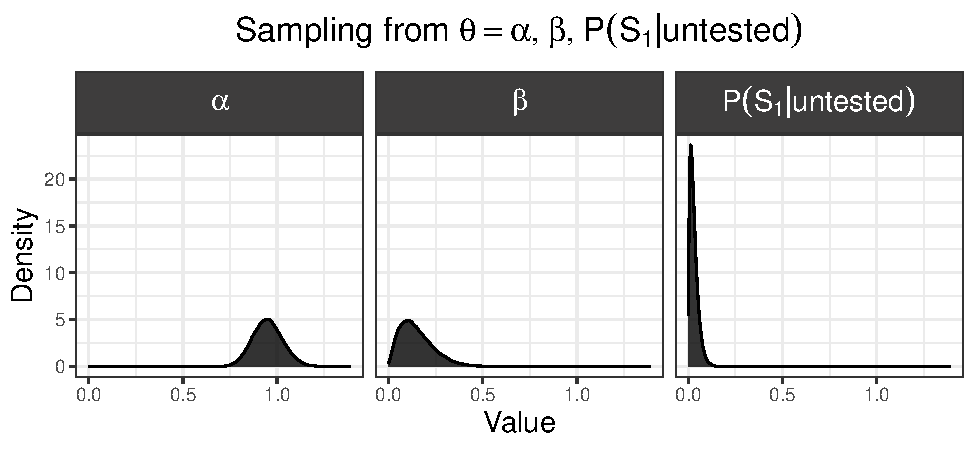
\includegraphics{thesis_files/figure-latex/unnamed-chunk-9-1} 

}

\caption{\label{fig:theta}}\label{fig:unnamed-chunk-9}
\end{figure}
\hypertarget{direct-prior-and-induced-prior-distributions-for-ps_0texttest_textuntested}{%
\subsection{\texorpdfstring{Direct Prior and Induced Prior Distributions for \(P(S_0|\text{test}_+,\text{untested})\)}{Direct Prior and Induced Prior Distributions for P(S\_0\textbar\textbackslash text\{test\}\_+,\textbackslash text\{untested\})}}\label{direct-prior-and-induced-prior-distributions-for-ps_0texttest_textuntested}}

Then, taking \(M(\theta)\), we can compute the induced distribution \(f_\phi^{induced}(M(\theta))\) and compare it to our prior on \(\phi\) from meta-analyses on the asymptomatic rate, \(f_\phi^{direct}(\phi)\) (\ref{fig:prior-induced}).
\begin{figure}

{\centering 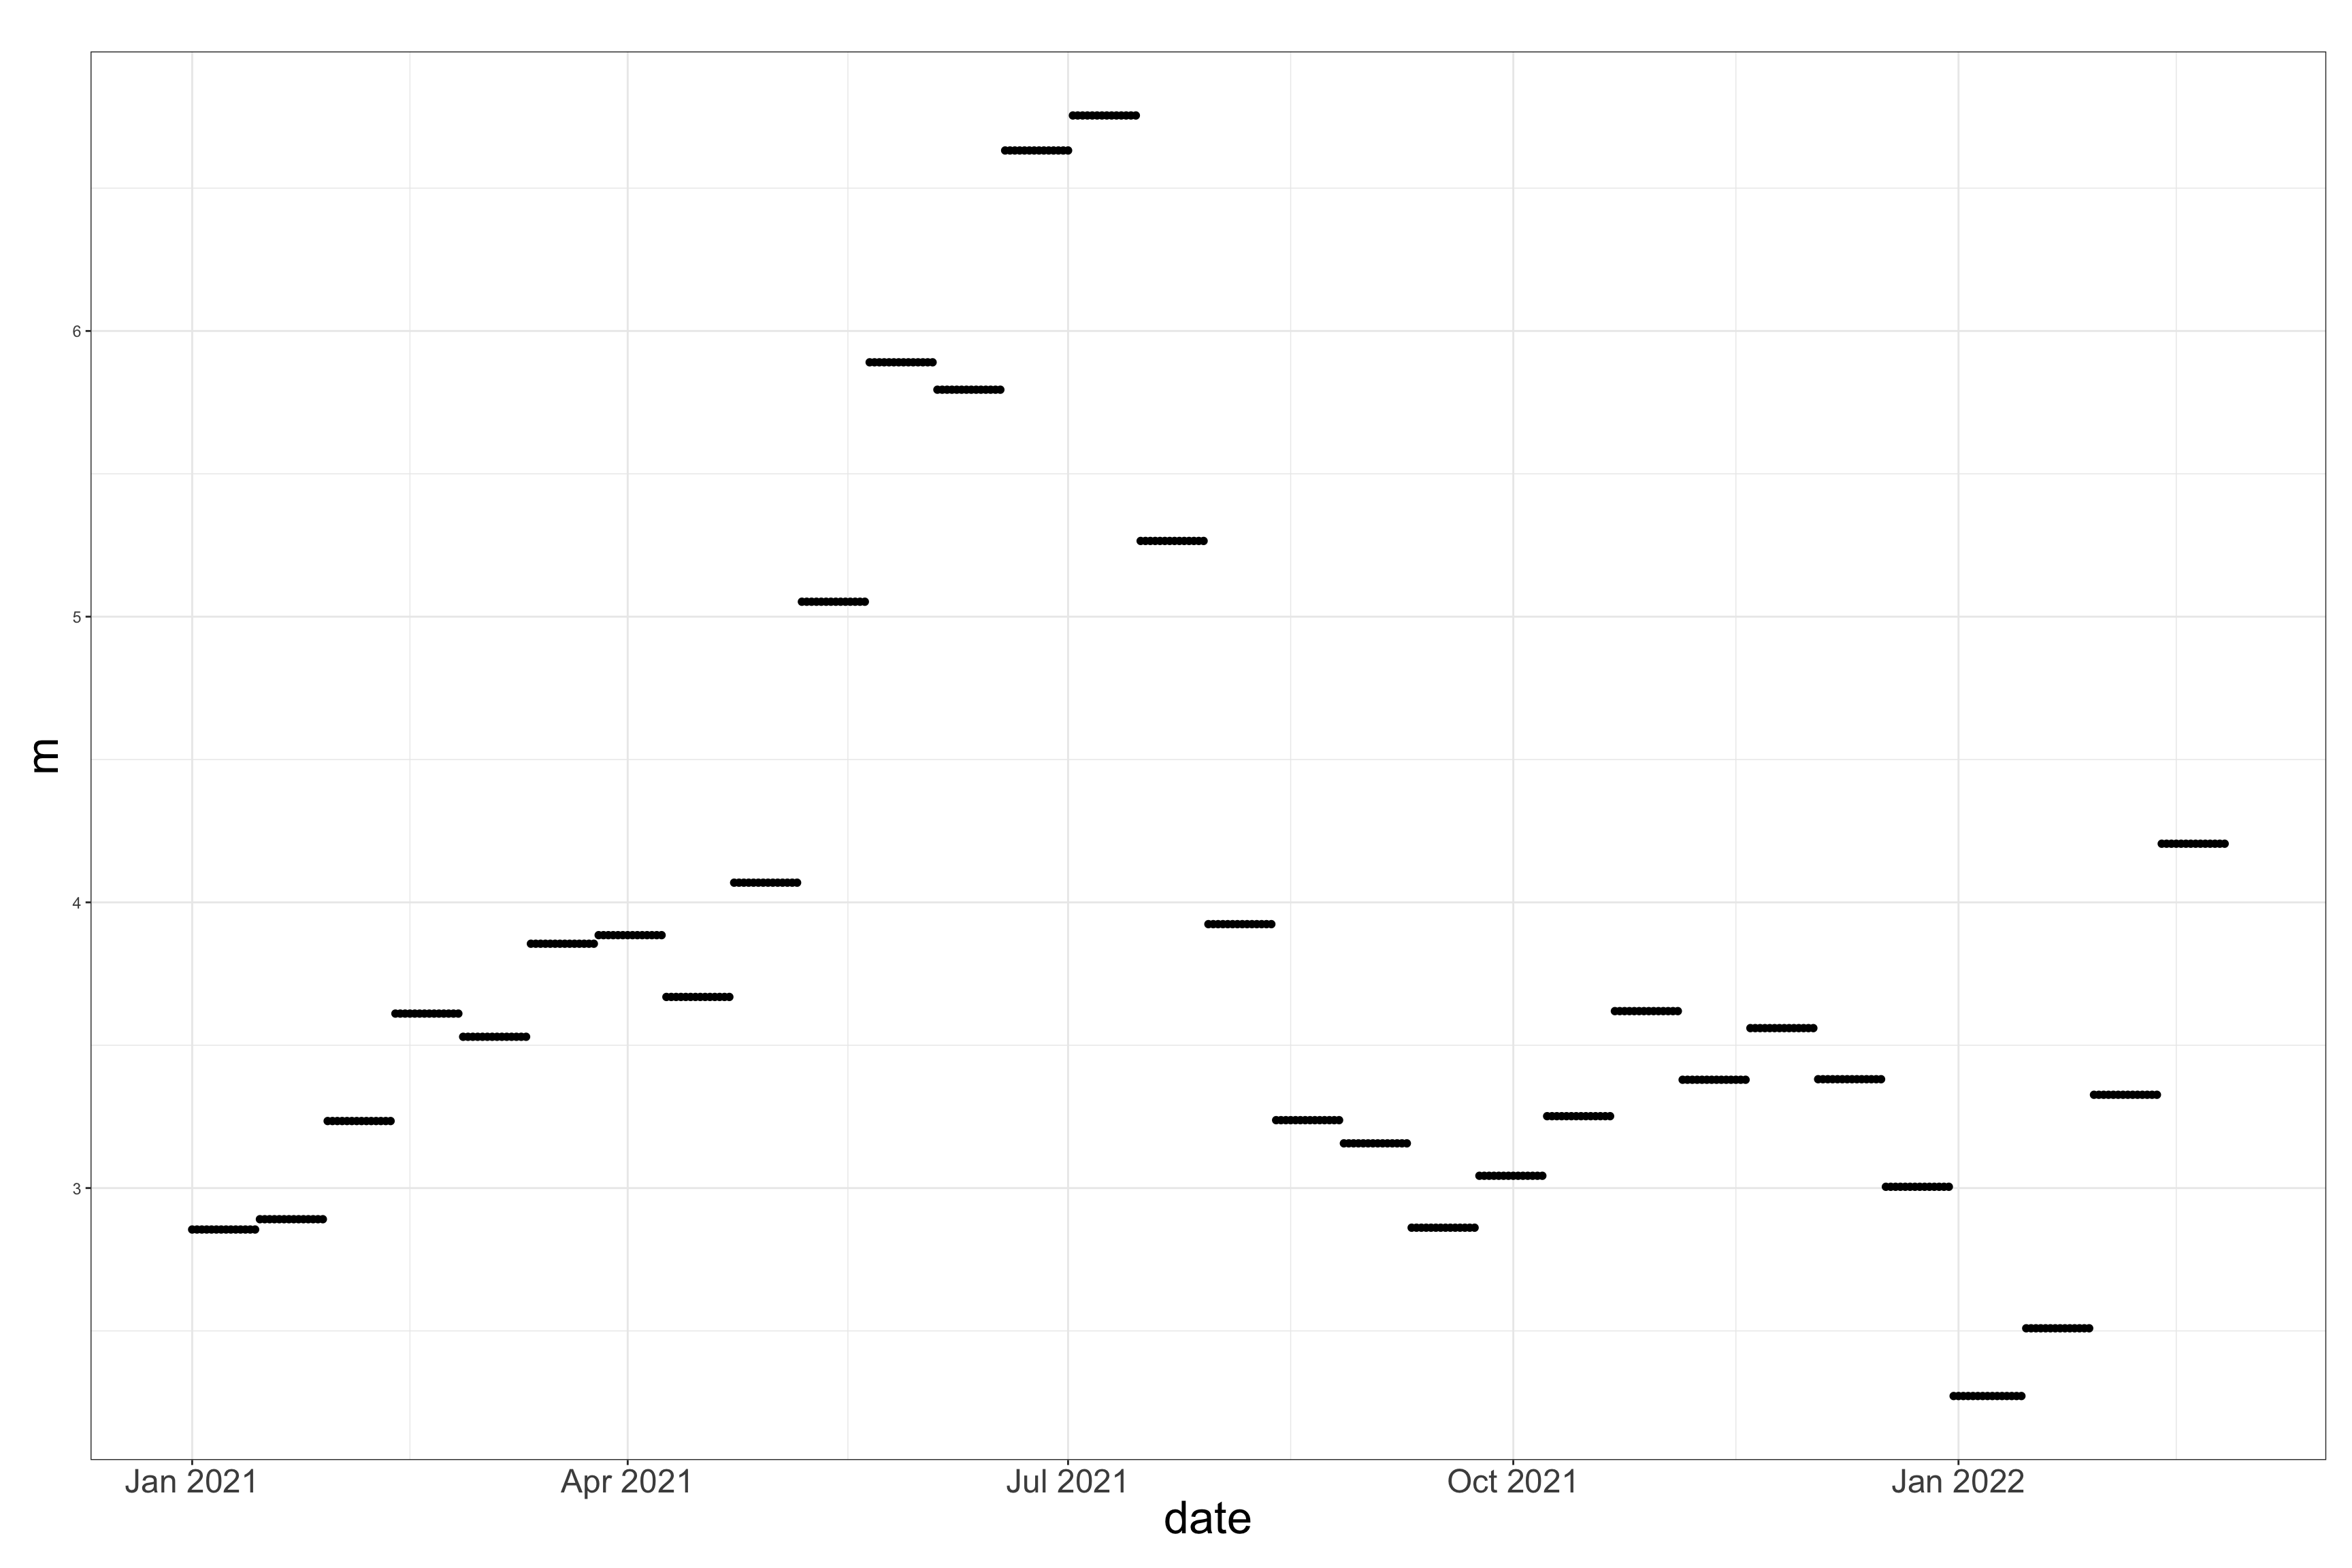
\includegraphics{thesis_files/figure-latex/unnamed-chunk-10-1} 

}

\caption{\label{fig:prior-induced}}\label{fig:unnamed-chunk-10}
\end{figure}
\newpage

\hypertarget{pooling}{%
\subsection{Pooling}\label{pooling}}

At this point, we want to obtain the logarithmically pooled distribution, denoted \(f^{pooled}\).

Now, as described in greater detail in the section on the \protect\hyperlink{logpooled}{Sampling-Importance-Resampling algorithm}, the weights are \(w_i = \left( \frac{f_\phi^{direct}(M(\theta_i))}{f_\phi^{induced}(M(\theta_i))} \right)^{1-\alpha}.\)

We perform a kernel density estimation to approximate the density of \(f_\phi^{induced}(\phi)\) at the coordinates \(\phi_1, \dots, \phi_M\). To compute \(f_\phi^{direct}(\phi)\), we can use the density function \(f_\phi^{direct}\).

Once we have these weights, we resample the \(\phi_1,\dots,\phi_M\) to obtain a sample from the target distribution \(t(\alpha) \Big( f^{induced}(M(\theta)) \Big)^{0.5} \Big( f^{direct} (M(\theta)) \Big)^{0.5}\), where \(t(\alpha)\) is the normalizing constant needed to make the pooled density valid. We resample \(\theta_1, \dots, \theta_k\) with the same weights to obtain the constrained distributions for the inputs.

We see the melded distributions and pre-melding distributions in Figure \ref{fig:melded}.
\begin{figure}

{\centering 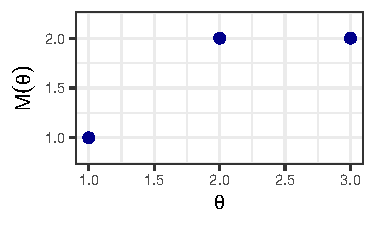
\includegraphics{thesis_files/figure-latex/unnamed-chunk-12-1} 

}

\caption{\label{fig:melded}}\label{fig:unnamed-chunk-12}
\end{figure}
Comparing the induced and direct priors on \(P(S_0| \text{test}_+, \text{untested})\) above, we see that although they have shared support, some values from the induced distribution we acquire by using \(M\) to generate values of \(\phi\) from sampled values of \(\theta\) are very unlikely to be in accordance with the information we know about the prevalence of SARS-CoV-2 asymptomatic infection. This is where Bayesian melding comes into play. Pooling these distributions enable us to take both the prior on \(f^{direct}\) from published analyses on asymptomatic infection, and the induced prior, \(f^{induced}\), into account to constrain the distributions of both the model inputs \(\theta = \{ \alpha, \beta, P(S_1 | \text{untested})\}\) and model output \(\phi = P(S_0|\text{test}_+, \text{untested})\) to be in accordance with both prior distributions. We then use these constrained distributions as inputs in the probabilistic bias analysis.

\newpage

\hypertarget{derivation}{%
\subsection{\texorpdfstring{Derivation of \(M\)}{Derivation of M}}\label{derivation}}

\indent We define \(\theta\) as the set of bias parameters \(\{P(S_1|\text{untested}), \alpha, \beta \}\). The parameters \(\alpha\) and \(\beta\) relate the observed overall test positivity rate to the test positivity rate we would obtain if we tested the asymptomatic and symptomatic partitions of the untested population. We define:
\begin{itemize}
\tightlist
\item
  \(\alpha = \dfrac{P(\text{test}_+|S_1,\text{untested})}{P(\text{test}_+|\text{tested})}\)
\item
  \(\beta = \dfrac{P(\text{test}_+|S_0,\text{untested})}{P(\text{test}_+|\text{tested})}\).
\end{itemize}
The parameter \(P(S_1|\text{untested})\) reflects the probability someone among the untested population has moderate to severe COVID-like symptoms.

We relate this set of parameters to the asymptomatic infection rate \(\phi = P(S_0|\text{test}_+, \text{untested})\) by the function \(M: \theta \to \phi\):
\begin{tcolorbox}
\vspace{2 mm}
\begin{align*}   
 M(\theta)  = \dfrac{\beta (1- P(S_1|\text{untested}))}{\beta(1- P(S_1|\text{untested})) + \alpha(P(S_1|\text{untested})} = P(S_0|\text{test}_+, \text{untested}).\\
\end{align*}
\end{tcolorbox}
In what follows, we show this equality holds.

\noindent Since we have \(\alpha = \frac{P(\text{test}_+|S_1, \text{untested})}{P(\text{test}_+|tested)}\) and \(\beta = \dfrac{P(\text{test}_+|S_0, \text{untested})}{P(\text{test}_+|tested)}\), we can write
\begin{align*}  &= \dfrac{\dfrac{P(\text{test}_+|S_0, \text{untested})}{P(\text{test}_+|tested)}(1 - P(S_1|\text{untested}))}{\dfrac{P(\text{test}_+|S_0, \text{untested})}{P(\text{test}_+|tested)}(1-P(S_1|\text{untested})) + \dfrac{P(\text{test}_+|S_1, \text{untested})}{P(\text{test}_+|tested)} P(S_1|\text{untested})}
\end{align*}
and cancelling out the term \(P(\text{test}_+|tested)\) we have

\[ = \dfrac{{P(\text{test}_+|S_0, \text{untested})}(1 - P(S_1|\text{untested}))}{P(\text{test}_+|S_0, \text{untested})(1-P(S_1|\text{untested})) + P(\text{test}_+|S_1, \text{untested}) P(S_1|\text{untested})}.\]

\noindent Since \(P(S_0|\text{untested}) = 1 - P(S_1|\text{untested})\),
\begin{align*} 
&=  \dfrac{{P(\text{test}_+|S_0, \text{untested})}P(S_0|\text{untested})}{P(\text{test}_+|S_0, \text{untested})P(S_0|\text{untested}) + P(\text{test}_+|S_1, \text{untested}) P(S_1|\text{untested})}.
\end{align*}
Applying the definition of conditional probability to the term
\(P(\text{test}_+|S_0, \text{untested})P(S_0|\text{untested})\) in the numerator,
\begin{align*}
&=
    \dfrac{\Big( \dfrac{P(\text{test}_+,S_0, \text{untested})}{P(S_0, \text{untested})} \Big) \Big(\dfrac{P(S_0, \text{untested})}{P(\text{untested})}\Big)}{P(\text{test}_+|S_0, \text{untested})P(S_0|\text{untested}) + P(\text{test}_+|S_1, \text{untested}) P(S_1|\text{untested})}\\ 
    &= \dfrac{\Big( \dfrac{P(\text{test}_+,S_0, \text{untested})}{P(S_0, \text{untested})} \Big) \Big(\dfrac{P(S_0, \text{untested})}{P(\text{untested})}\Big)}{P(\text{test}_+|S_0, \text{untested})P(S_0|\text{untested}) + P(\text{test}_+|S_1, \text{untested}) P(S_1|\text{untested})}\\
    &=  \dfrac{\dfrac{P(\text{test}_+,S_0, \text{untested})}{P(\text{untested})}}{P(\text{test}_+|S_0, \text{untested})P(S_0|\text{untested}) + P(\text{test}_+|S_1, \text{untested}) P(S_1|\text{untested})}\\
    &=  \dfrac{{P(\text{test}_+,S_0|\text{untested})}}{P(\text{test}_+|S_0, \text{untested})P(S_0|\text{untested}) + P(\text{test}_+|S_1, \text{untested}) P(S_1|\text{untested})}.
\end{align*}
\noindent We can substitute this result in for the \(P(\text{test}_+|S_0, \text{untested})P(S_0|\text{untested})\) term in the denominator to yield
\begin{align*}
  &=  \dfrac{{P(\text{test}_+,S_0|\text{untested})}}{P(\text{test}_+,S_0|\text{untested}) + P(\text{test}_+|S_1, \text{untested}) P(S_1|\text{untested})} \hspace{ 20 mm }
\end{align*}
With same reasoning, we can simplify
\begin{align*}
P(\text{test}_+|S_1, \text{untested})P(S_1|\text{untested}) = P(S_1, \text{test}_+|\text{untested}),
\end{align*} giving us
\begin{align*}
  &=  \dfrac{{P(\text{test}_+,S_0|\text{untested})}}{P(\text{test}_+,S_0|\text{untested}) +  P(S_1, \text{test}_+|\text{untested})} \hspace{45 mm }\\ 
   &=  \dfrac{{P(\text{test}_+,S_0|\text{untested})}}{P(\text{test}_+|\text{untested}) } \\
   &= \dfrac{\dfrac{P(S_0, \text{test}_+, \text{untested})}{P(\text{untested})}}{ \dfrac{P(\text{test}_+,\text{untested})}{P(\text{untested})}} \\ 
  &=\dfrac{P(S_0, \text{test}_+, \text{untested})}{P(\text{test}_+,\text{untested})} \\
  &= P(S_0 |\text{test}_+, \text{untested}).
\end{align*}
\noindent Hence, we have
\begin{align*}
P(S_0 |\text{test}_+, \text{untested}) = \dfrac{\beta (1- P(S_1|\text{untested}))}{\beta(1- P(S_1|\text{untested})) + \alpha(P(S_1|\text{untested})}
\end{align*}
\noindent as desired.
\qed

\newpage

\hypertarget{sampling-importance-resampling-algorithm}{%
\section{\texorpdfstring{Sampling-Importance-Resampling Algorithm \label{sampling}}{Sampling-Importance-Resampling Algorithm }}\label{sampling-importance-resampling-algorithm}}

\hypertarget{overview}{%
\subsection{Overview}\label{overview}}

~~~The Sampling-Importance-Resampling Algorithm, introduced in Rubin (1987), is a non-iterative method for approximating a sample from a target probability density function \(f\). This algorithm is fundamental to the implementation of Bayesian melding.

The two main steps are the sampling step and importance resampling step. We have two (generally distinct) sample sizes, where \(m\) is the initial sample size and \(r\) is the resample size.

In the sampling step, we draw an independent and identically distributed sample of size \(m\) from \(g\), \(Y_1, Y_2, \dots, Y_m\). Then, we compute weights \(h(Y)\) such that \(g \cdot h \propto f\). That is, we set the weights

\[w_i = h(Y_i) = \dfrac{\frac{f(Y_i) } {g(Y_i)} }{\sum_{i=1}^m\frac{f(Y_i) } {g(Y_i)} }.\]

We resample with these defined weights to obtain a sample of size \(r\) from \(Y_1, Y_2, \dots, Y_m\). We denote this resample \(Z_1,\dots, Z_r\). With these weights, \(Z_1,\dots, Z_r\) is approximately a sample from \(f\).

The method is most efficient when \(g\) is a good approximation of \(f\). The relationship between the sample size \(m\) and resample size \(r\) also has implications for the quality of the approximation. The algorithm generates independent and identically distributed samples as \(m/r \to \infty\), but in most applications \(m/r\) between 10 and 20 is appropriate (Rubin, Gelman, \& Meng, 2004). The practical implications of this choice are discussed \protect\hyperlink{presamp}{later in this section}.

To better understand the use of this algorithm, we provide a proof that formally relates the choice of \(g\), weights \(h\), and the target distribution \(f\). We then follow up with a couple concrete examples where there is a closed formed solution to visualize how the algorithm works in practice.

\hypertarget{proof}{%
\subsection{Proof that Algorithm Obtains Approximate Sample from Target Distribution}\label{proof}}

To gain further insight into how sampling with weights
\(w_i = \left( \frac{f_\phi^{direct}(M(\theta_i))}{f_\phi^{induced}(M(\theta_i))} \right)^{0.5}\)
approximates a sample from the target distribution the logarithmically pooled distribution \(f^{pooled}\), we first prove a more general result.
\begin{tcolorbox}
Suppose we sample $Y_1, Y_2, \dots, Y_m$ independently and identically distributed with probability density function  $g$ and compute the weights
\[ w_i =\dfrac{h(Y_i)}{\sum_{i=1}^mh(Y_i) }\]
for some nonnegative function $h$ defined on the support of $Y$.

If  we sample $Z_1, \dots, Z_r$ from the discrete distribution $Y_1,\dots, Y_m$ such that 

\[ P(Z = Y_i) = \dfrac{h(Y_i)}{\sum_{i=1}^mh(Y_i) } = w_i ,\]
then $Z_1, \dots, Z_r$ is approximately a sample with density proportional to $h \cdot g$.

\end{tcolorbox}
\vspace{5 mm}

Since \(Z\) is sampled from \(Y\), we have
\[ P(Z \leq x ) = \sum_{z_i \leq x} P(Z=z_i) = \sum_{Y_i \leq x} P(Z=Y_i) .\]

We can take this sum to be over all possible values of \(Y\) by including the indicator function \(\mathbb{I} (Y_i \leq x)\), yielding
\[  = \sum_{i = 1}^m P(Z=y_i)\;\;\mathbb{I} (Y_i \leq x).  \]
and since \(P(Z=Y_i) = \dfrac{h(Y_i)}{\sum_{i=1}^mh(Y_i) }\) by definition we have
\begin{align*} 
&= \sum_{i = 1}^m \dfrac{h(Y_i)}{\sum_{i=1}^mh(Y_i) }  \;\;\mathbb{I} (Y_i \leq x)   \\
&=  \left( \dfrac{1}{ {\sum_{i=1}^mh(Y_i) }} \right) {\sum_{i=1}^mh(Y_i) }  \;\;\mathbb{I} (Y_i \leq x)   \\
&=   \dfrac{ {\sum_{i=1}^mh(Y_i) }  \;\;\mathbb{I} (Y_i \leq x) }{\sum_{i=1}^mh(Y_i) } \\
&=   \dfrac{ \frac 1m {\sum_{i=1}^mh(Y_i) }  \;\;\mathbb{I} (Y_i \leq x) }{\frac 1m \sum_{i=1}^mh(Y_i) }. \\
\end{align*}
Now, we need the Weak Law of Large Numbers. That is, if we have a sequence of random variables \(X_1, X_2, \dots\) with finite variance, then,
\[ \lim_{n \to \infty} \left( \frac{1}{n} \sum_{i=1}^n X_i \right)  = E(X_i). \]

Applying this law to both the numerator and denominator, we obtain
\begin{align*}  \lim_{m \to \infty} \left( \dfrac{ \frac 1m {\sum_{i=1}^mh(Y_i) }  \;\;\mathbb{I} (Y_i \leq x) }{\frac 1m \sum_{i=1}^mh(Y_i) } \right) &= \dfrac{ E_g[ h(Y) \;\; \mathbb I (Y \leq x) ]  }{ E_g[ h(Y) ]  }\\
&= \dfrac{\int_{-\infty}^\infty h(y) \;\; \mathbb I (y \leq x) \; g(y) \; dy}{\int_{-\infty}^\infty h(y) \, g(y) \;dy}\\
&= \dfrac{\int_{-\infty}^x h(y) \, g(y) dy}{\int_{-\infty}^\infty h(y) \, g(y) \;dy}\\
&\propto \int_{-\infty}^x h(y) \, g(y) dy. 
\end{align*}
It follows that the probability density function of \(Z\) is proportional to \(h \cdot g\).

\vspace{3 mm}

\qed

It is easiest to understand the Sampling-Importance-Resampling Algorithm when the resampled distribution has a closed form, which we can see in the following two examples.

\newpage

\hypertarget{example-1}{%
\subsubsection{Example 1:}\label{example-1}}

Suppose \(Y \sim Exp(\lambda)\), so we have the PDF \(f_Y(y) = \lambda e^{-\lambda y}\), and we sample \(Z_1,\dots,Z_r\) from \(Y_1, \dots, Y_m\) with weights direction proportional to \(X\), that is, \(h(Y) = Y\).

Then \(Z_1,\dots Z_r\) is approximately a sample from \(h(x) \; f_Y(y) = y \; \lambda e^{-\lambda y}\).

From the PDF of the gamma distribution, \(\dfrac{\beta^\alpha}{\Gamma(\alpha) }y^{\alpha - 1} e^{-\beta y}\) we can recognize that \(y \cdot e^{-\lambda y}\) corresponds to the gamma distribution with \(\alpha = 2\) and \(\beta = \lambda\).

We can see this result by considering \(Y\) before and after resampling below (Figure \ref{fig:ex1}).
\begin{figure}

{\centering 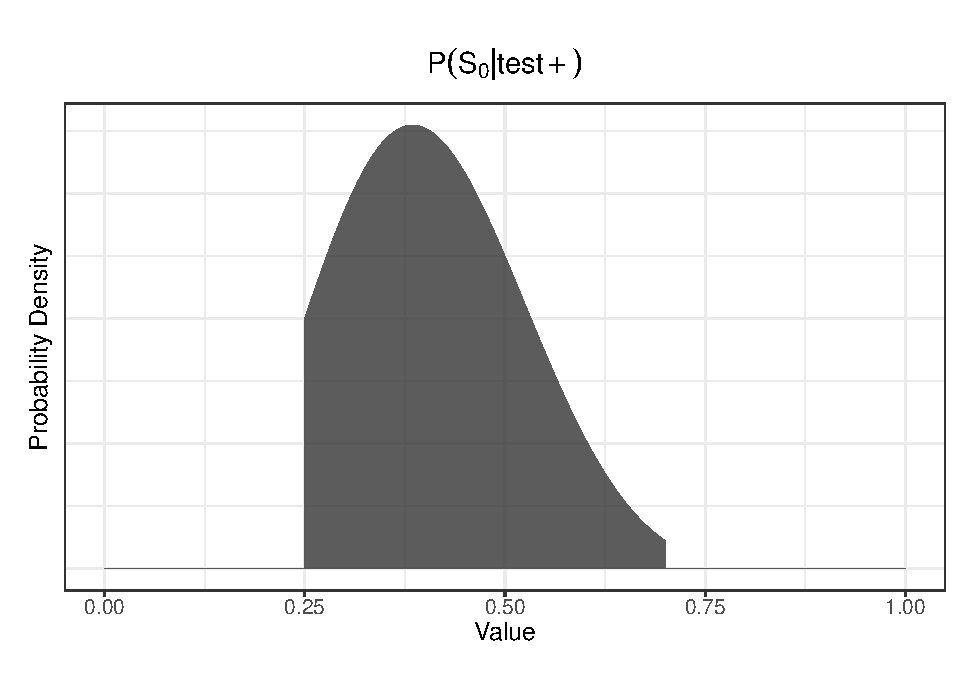
\includegraphics{thesis_files/figure-latex/unnamed-chunk-13-1} 

}

\caption{\label{fig:ex1}}\label{fig:unnamed-chunk-13}
\end{figure}
Then, we can see that the PDF of the the gamma distribution with \(\alpha = 2\) and \(\beta = \lambda\) corresponds to the post-sampling distribution as expected (Figure \ref{fig:ex12}).
\begin{figure}

{\centering 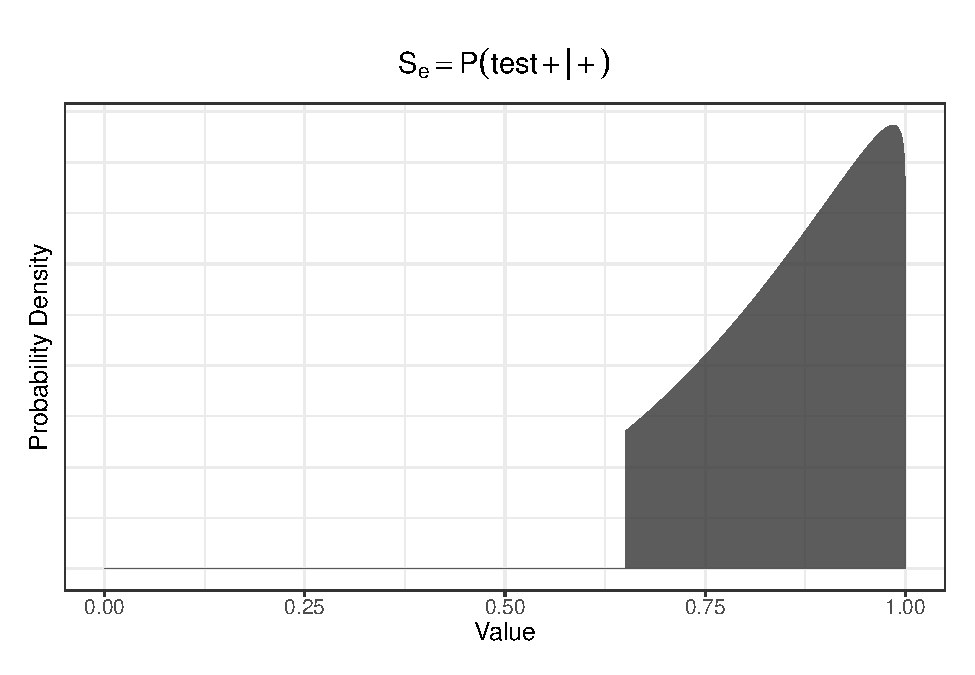
\includegraphics{thesis_files/figure-latex/unnamed-chunk-14-1} 

}

\caption{\label{fig:ex12}}\label{fig:unnamed-chunk-14}
\end{figure}
\newpage

\hypertarget{example-2}{%
\subsubsection{Example 2:}\label{example-2}}

Similarly, again suppose \(Y \sim Exp(\lambda)\), so \(f_Y(y) = \lambda e^{-\lambda y}\). However, now we sample with weights defined by \(h(y)= e^{-\lambda y}\).
Then our sample \(Z_1,\dots,Z_r\) is approximately a sample from
\begin{align*} 
h(y) \; f_Y(y) &=   e^{-\lambda y} \cdot \lambda e^{-\lambda y}\\
&= \ e^{-2 \lambda y}  
\end{align*}
which is proportional to the exponential distribution with parameter \(2\lambda\).

The distributions before and after resampling are shown in Figure \ref{fig:ex2}.
\begin{figure}

{\centering 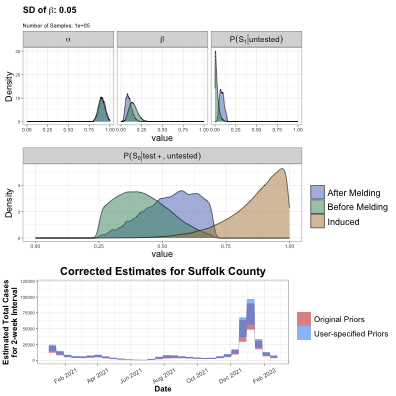
\includegraphics{thesis_files/figure-latex/unnamed-chunk-15-1} 

}

\caption{\label{fig:ex2}}\label{fig:unnamed-chunk-15}
\end{figure}
and then plotting the PDF of the exponential distribution with parameter \(2\lambda\) we can see the correspondence to the post-sampling distribution (Figure \ref{fig:ex22}).
\begin{figure}

{\centering 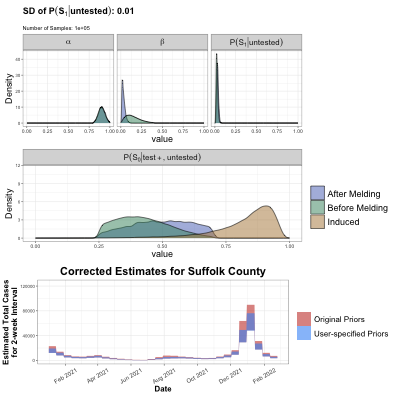
\includegraphics{thesis_files/figure-latex/unnamed-chunk-16-1} 

}

\caption{\label{fig:ex22}}\label{fig:unnamed-chunk-16}
\end{figure}
\newpage

\hypertarget{logpooled}{%
\subsection{Obtaining Logarithmic Pooled Distribution with the Sampling-Importance-Resampling Algorithm}\label{logpooled}}

As outlined in Carvalho, Villela, Coelho, \& Bastos (2023), we can formally define logarithmic pooling as follows.

If we have a set of densities \(\{ f_1(\phi), f_2(\phi), \ldots, f_n(\phi)\}\) and corresponding pooling weights \(\boldsymbol{\alpha}=\{\alpha_1, \alpha_2, \ldots, \alpha_n\}\), then the pooled density is

\[ t(\boldsymbol{\alpha}) \prod_{i=0}^n f_i(\phi)^{\alpha_i}\] where \(t(\boldsymbol{\alpha})\) is the normalizing constant \(t(\boldsymbol{\alpha}) = \dfrac{1}{ \int_{\Phi}\prod_{i=0}^n f_i(\phi)^{\alpha_i} d\phi}\) to ensure the pooled density is a valid probability density.

The case for this work is more simple: we only have two densities we wish to pool, \(f_\phi^{induced}\) and \(f_\phi^{direct}\), and we assign them equal weights by letting \(\boldsymbol{\alpha} = \{.5, .5\}\). This yields

\[f^{pooled}(\phi) = t(\boldsymbol \alpha) \left( f^{induced} (\phi) \right)^{0.5} \left( f^{direct} (\phi) \right)^{0.5}.\]

Since our target distribution is \(t(\boldsymbol \alpha) \left( f^{induced} (\phi) \right)^{0.5} \left( f^{direct} (\phi) \right)^{0.5}\), and we have a sample from \(f^{induced}\), we compute the weights such that
\begin{align*} w_i &\propto \dfrac{ \left( f^{induced} (\phi_i) \right)^{0.5} \left( f^{direct} (\phi_i) \right)^{0.5} } {f^{induced}(\phi_i)} \\
&=  \dfrac{ \left( f^{direct} (\phi_i) \right)^{0.5} } {\left( f^{induced} (\phi_i) \right)^{0.5} } \\
&=   \left( \dfrac{  f^{direct} (\phi_i) } { f^{induced} (\phi_i) }  \right)^{0.5}. \\
\end{align*}
Sampling from \(f^{induced}\) with these weights will yield a sample with approximately the target density \(t(\alpha) \left(f^{induced} (\phi) \right)^{0.5} \left( f^{direct} (\phi)\right)^{0.5}\) from the result in the \protect\hyperlink{proof}{previous section}.

\hypertarget{presamp}{%
\subsection{Implications of the Sample Size and Resample Size}\label{presamp}}

When we have an initial sample of size \(m\) from \(g\), denoted \(Y_1,\dots,Y_m\), and take a weighted sample of size \(r\), \(Z_1,\dots,Z_r\), the choices of \(m\) and \(r\) can have notable effects on the estimated distribution of the resample. In particular, when the sample size and resample size do not differ substantially, it becomes more likely that we will sample some element of \(Y_1,\dots,Y_m\) more than once. This can result in irregularities in the estimated distribution of \(Z_1,\dots,Z_r\). We see this in \ref{fig:prepostsamp} when the ratio of \(m/r\) is closer to 1, while the problem reduces as we increase the sample size \(m\) compared to the posterior (resample) size \(r\).
\begin{figure}

{\centering 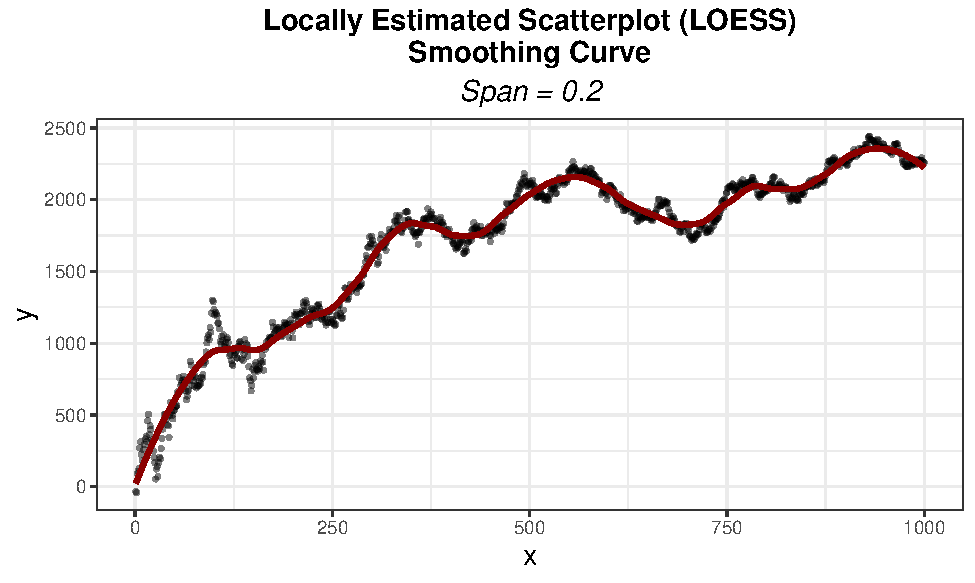
\includegraphics[width=0.45\linewidth]{thesis_files/figure-latex/unnamed-chunk-18-1} 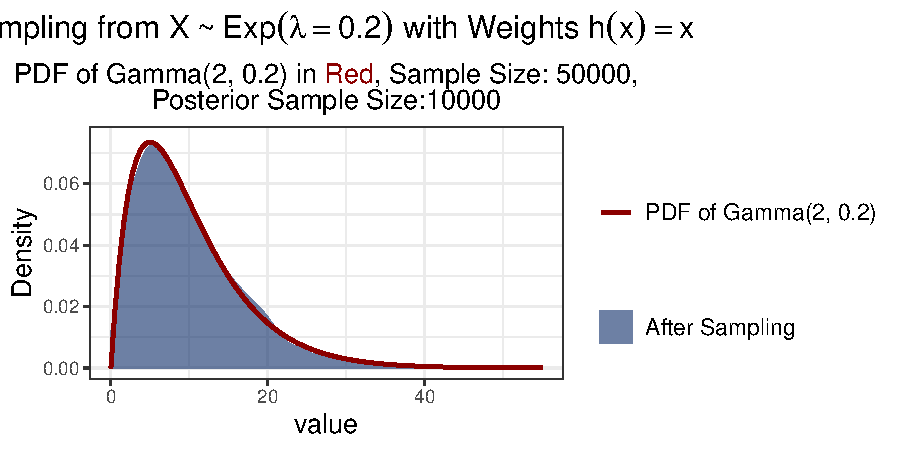
\includegraphics[width=0.45\linewidth]{thesis_files/figure-latex/unnamed-chunk-18-2} 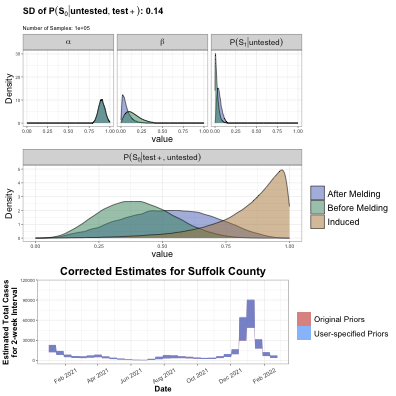
\includegraphics[width=0.45\linewidth]{thesis_files/figure-latex/unnamed-chunk-18-3} 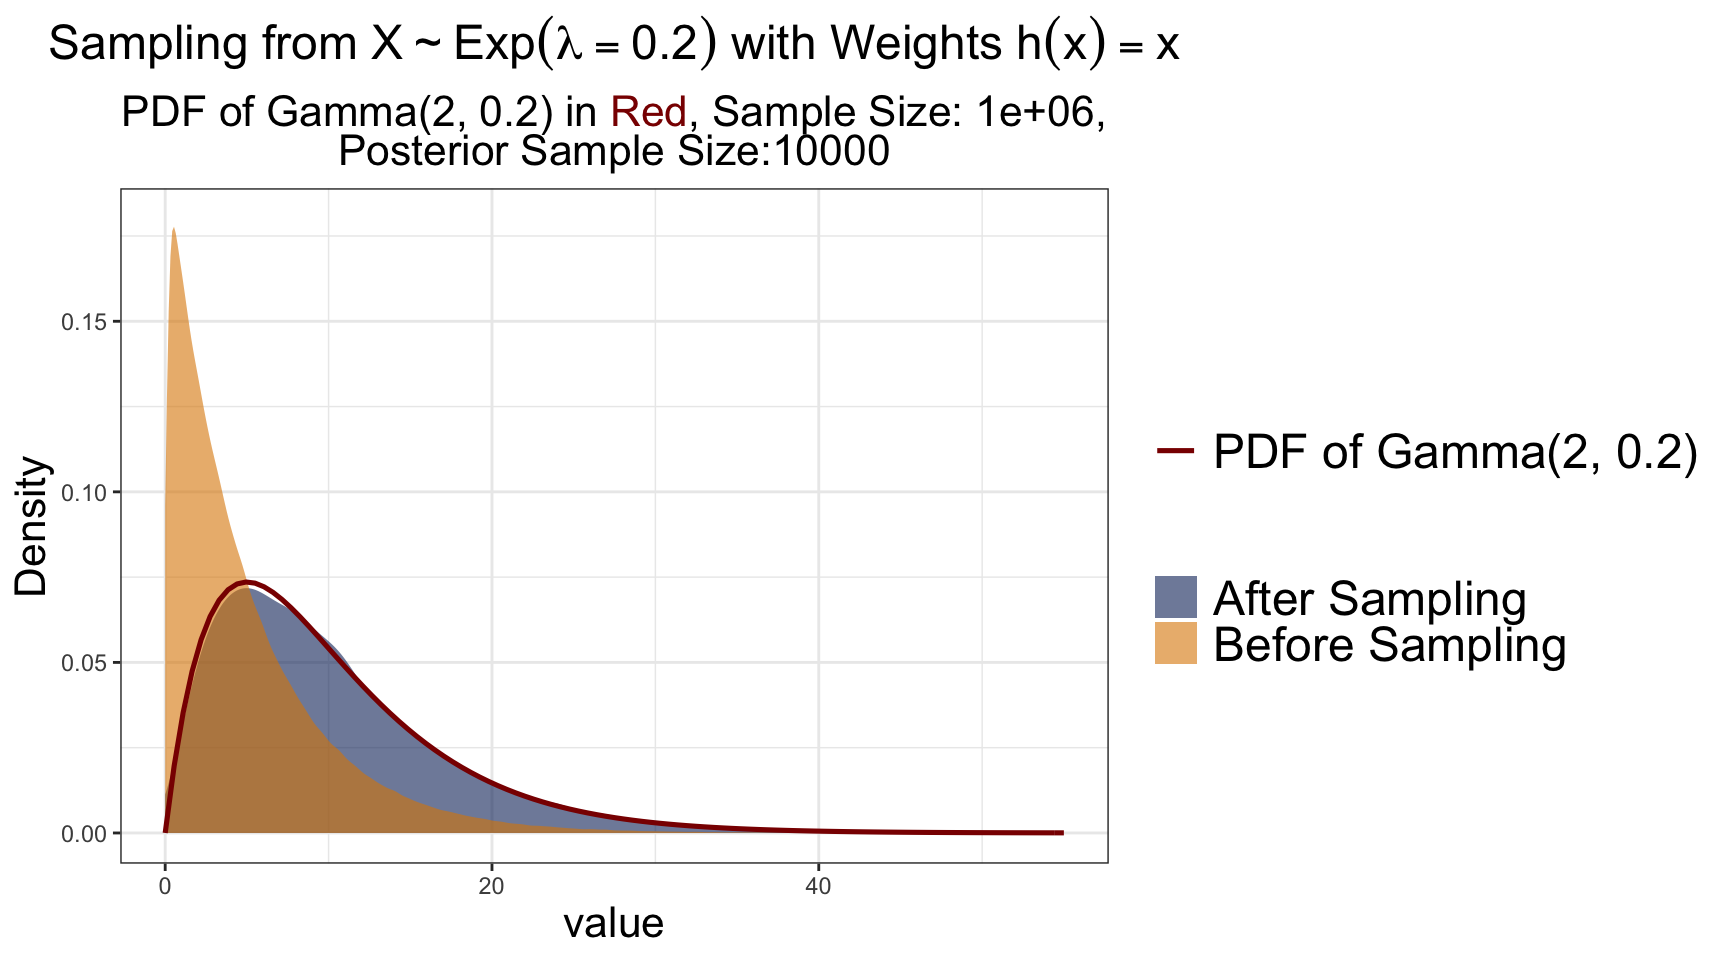
\includegraphics[width=0.45\linewidth]{thesis_files/figure-latex/unnamed-chunk-18-4} 

}

\caption{\label{fig:prepostsamp}}\label{fig:unnamed-chunk-18}
\end{figure}
When using the Sampling-Importance-Resampling algorithm to obtain the logarithmically pooled distribution, see the effect of this choice has a major impact when we are melding truncated distributions. The pooled distribution is only defined on the intersection of the supports of the distributions being pooled. Truncation, then, can limit the choices of \(Y_1,\dots, Y_m\) we take when resampling, which can lead to substantial irregularities in the resulting estimated pooled distribution (Figure \{fig:trunc\}).
\begin{verbatim}
Arguments to get_melded:
$alpha_mean
[1] 0.95

$alpha_sd
[1] 0.08

$alpha_bounds
[1] NA

$beta_mean
[1] 0.15

$beta_sd
[1] 0.09

$beta_bounds
[1] NA

$s_untested_mean
[1] 0.03

$s_untested_sd
[1] 0.0225

$s_untested_bounds
[1] NA

$p_s0_pos_mean
[1] 0.4

$p_s0_pos_sd
[1] 0.1225

$p_s0_pos_bounds
[1] 0.25 0.70

$pre_nsamp
[1] 10000

$post_nsamp
[1] 10000
\end{verbatim}
\begin{verbatim}
Arguments to get_melded:
$alpha_mean
[1] 0.95

$alpha_sd
[1] 0.08

$alpha_bounds
[1] NA

$beta_mean
[1] 0.15

$beta_sd
[1] 0.09

$beta_bounds
[1] NA

$s_untested_mean
[1] 0.03

$s_untested_sd
[1] 0.0225

$s_untested_bounds
[1] NA

$p_s0_pos_mean
[1] 0.4

$p_s0_pos_sd
[1] 0.1225

$p_s0_pos_bounds
[1] 0.25 0.70

$pre_nsamp
[1] 1e+05

$post_nsamp
[1] 10000
\end{verbatim}
\begin{verbatim}
Arguments to get_melded:
$alpha_mean
[1] 0.95

$alpha_sd
[1] 0.08

$alpha_bounds
[1] NA

$beta_mean
[1] 0.15

$beta_sd
[1] 0.09

$beta_bounds
[1] NA

$s_untested_mean
[1] 0.03

$s_untested_sd
[1] 0.0225

$s_untested_bounds
[1] NA

$p_s0_pos_mean
[1] 0.4

$p_s0_pos_sd
[1] 0.1225

$p_s0_pos_bounds
[1] 0.25 0.70

$pre_nsamp
[1] 1e+06

$post_nsamp
[1] 10000
\end{verbatim}
\begin{figure}

{\centering 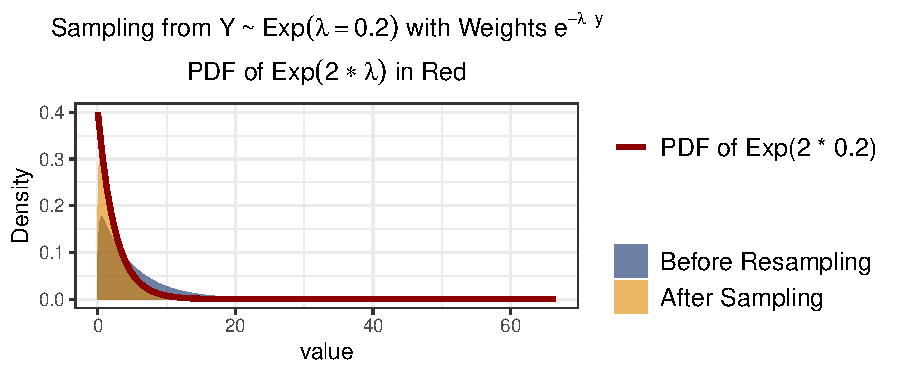
\includegraphics[width=0.5\linewidth]{thesis_files/figure-latex/unnamed-chunk-19-1} 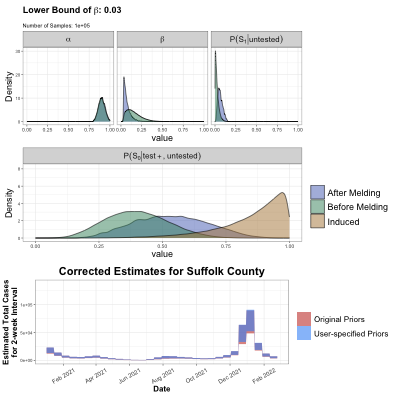
\includegraphics[width=0.5\linewidth]{thesis_files/figure-latex/unnamed-chunk-19-2} 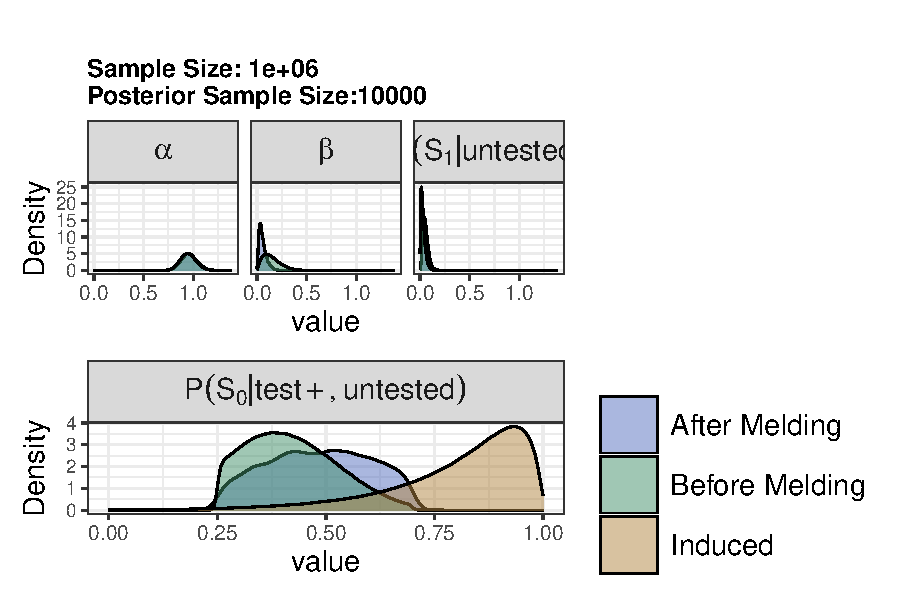
\includegraphics[width=0.5\linewidth]{thesis_files/figure-latex/unnamed-chunk-19-3} 

}

\caption{\label{fig:trunc}}\label{fig:unnamed-chunk-19}
\end{figure}
\newpage

\hypertarget{loess-smoothing}{%
\section{LOESS Smoothing}\label{loess-smoothing}}

\hypertarget{introduction}{%
\subsection{Introduction}\label{introduction}}

Locally estimated scatterplot smoothing (LOESS) fits a collection of local regression models to obtain a smooth curve through the observed data (Figure \ref{fig:loess}). It is highly flexible in the sense that we do not have to specify the functional relationship between the predictor and response variable for the entire range of the predictor, which may be impossible in various settings. It is particularly useful when working with time series data with substantial noise.
\begin{figure}

{\centering 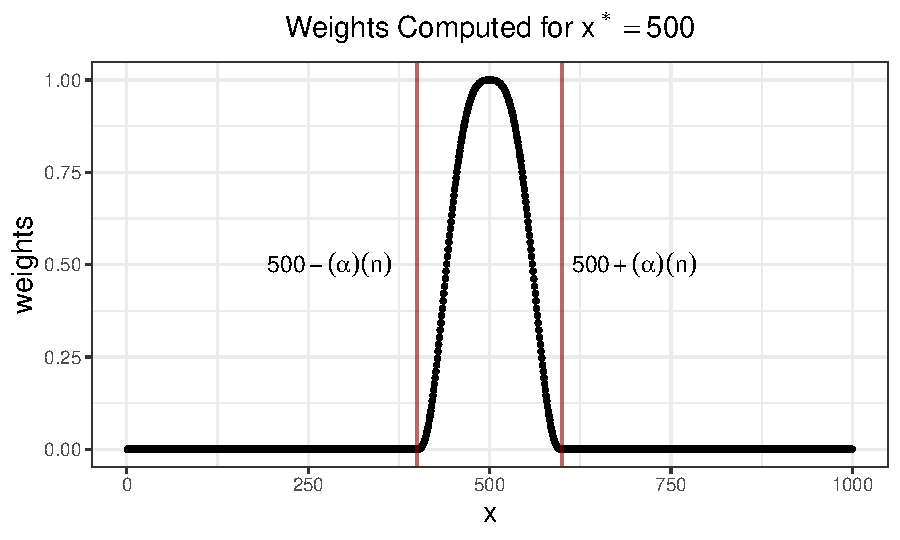
\includegraphics{thesis_files/figure-latex/unnamed-chunk-20-1} 

}

\caption{\label{fig:loess}LOESS curve fitted with  a span of 0.2. }\label{fig:unnamed-chunk-20}
\end{figure}
To perform LOESS smoothing, we estimate a set of local regressions (Chambers, 1997). To do this, we must specify the span; this smoothing parameter is the fraction of the data that is used for the local polynomial fit. With a smaller span, the resulting curve will fit the trends more closely, while a larger span reflects broader trends (Figure \ref{fig:smooth-spans}).
\begin{figure}

{\centering 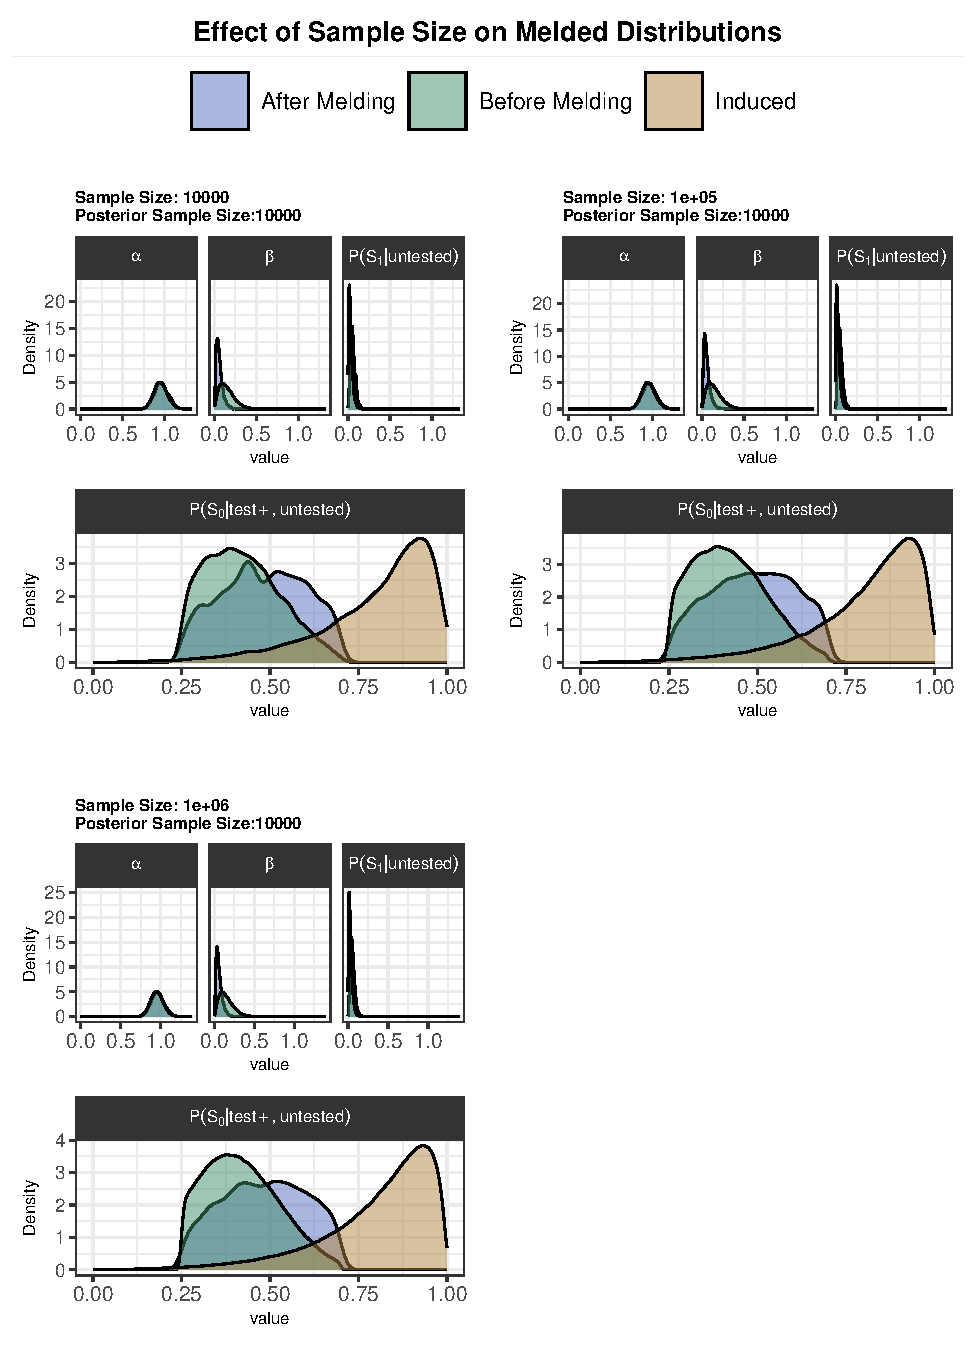
\includegraphics{thesis_files/figure-latex/unnamed-chunk-21-1} 

}

\caption{\label{fig:smooth-spans}}\label{fig:unnamed-chunk-21}
\end{figure}
\hypertarget{fitting-the-loess-curve}{%
\subsection{Fitting the LOESS Curve}\label{fitting-the-loess-curve}}

To introduce some notation for the model at hand, we have a dependent variable \(\mathbf y\) and independent variable \(\mathbf x\), where \(\mathbf y\) and \(\mathbf x\) are related by some unknown function \(g\), that is, \(y = g(x) + \boldsymbol \epsilon\)\footnote{Recall we use bold type for vectors, e.g., \(\mathbf x \in \mathbb R^n\) is a vector with observations \(x_i \in \mathbb R\).}. When we want to use LOESS smoothing to estimate \(g\), often this function is complex, so we break up the problem into estimating a set of local regressions.

To obtain a predicted value \(\hat g(x^*)\) for a particular value of the independent variable \(x^*\), we fit a polynomial with greatest weight placed on points in the neighborhood of \(x^*\), where the width of this neighborhood is defined by the choice of smoothing span. Let \(\alpha \in (0,1]\) denote the chosen smoothing span.

For a particular value of \(x^*\), we estimate the predicted value \(\hat g(x^*)\) by fitting a local regression. We first compute the weights by computing the vector of distances from this point \(x^*\), that is,

\[\Delta (x^*) = |\mathbf x -x^* | \]

We define \(q = \text{floor}(\alpha n)\), and take \(\Delta_q(x^*) \in \mathbb R\) to be the \(q^th\) smallest distance of \(\Delta (x^*)\).

The vector of weights is then
\[T(\Delta(x^*), \Delta_q(x^*))\]

where \(T\) is the tricube weight function given by

\[
T(x) = \begin{cases} (1-(x)^3)^3 \hspace{9 mm}  \text{ for } |x| < 1\\
0  \hspace{25 mm} \text{ for |x| } \geq 1 \end{cases}.
\]
Essentially, this process gives weight to points in the neighborhood of \(x^*\). Consider \(x^* = 500\) and \(\text{smoothing span} = \alpha = .2\).

Then the weights we obtain are given in Figure \ref{fig:weights}.
\begin{figure}

{\centering 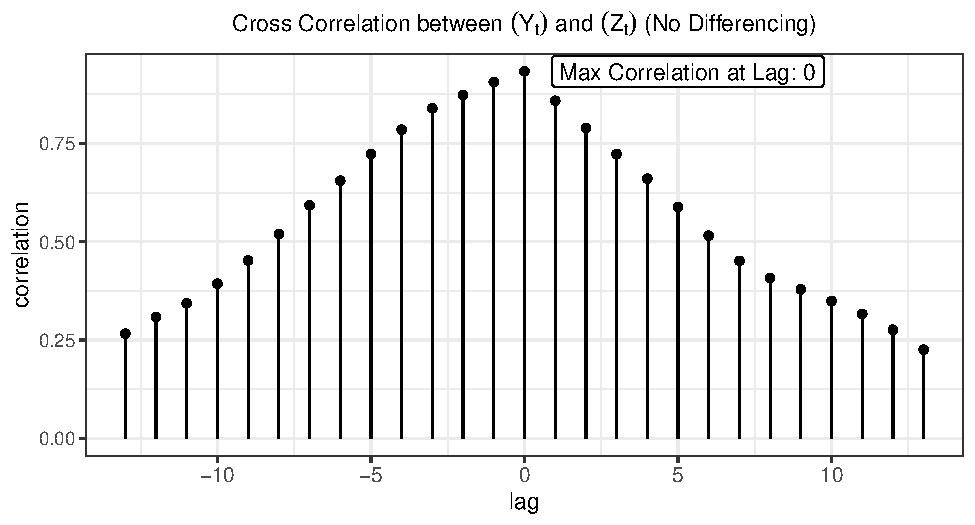
\includegraphics{thesis_files/figure-latex/unnamed-chunk-22-1} 

}

\caption{\label{fig:weights} The only values with nonzero weights are those within the interval $(500 - \alpha (n), 500 - \alpha (n))$. That is, the proportion $\alpha$ of the data points closest to $x^*$ will have nonzero weights.}\label{fig:unnamed-chunk-22}
\end{figure}
\newpage

We fit a linear regression with polynomial terms, typically with degree up to 2, with these weights. For example, fitting the model for this same \(x^*=500\), we obtain the polynomial in Figure \ref{fig:ex-poly}.
\begin{flushleft}
\begin{figure}

{\centering 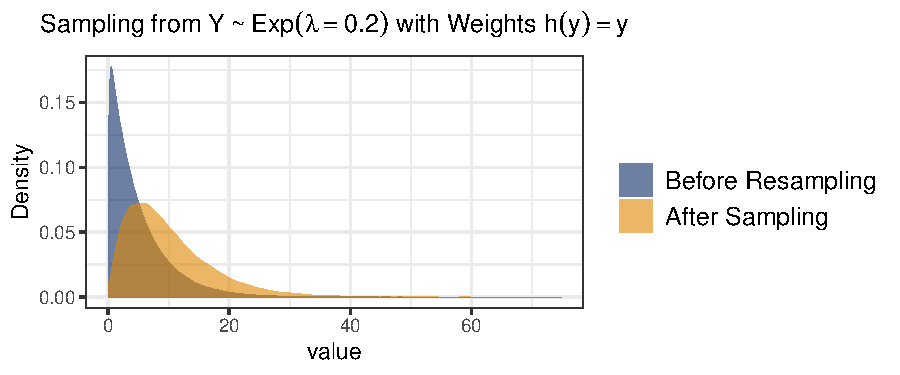
\includegraphics{thesis_files/figure-latex/unnamed-chunk-23-1} 

}

\caption{\label{fig:ex-poly}}\label{fig:unnamed-chunk-23}
\end{figure}
\end{flushleft}
By fitting the model for every point in \(\mathbf x\), we obtain the smoothed line shown in red in Figure \ref{fig:loess-all}.
\begin{figure}

{\centering 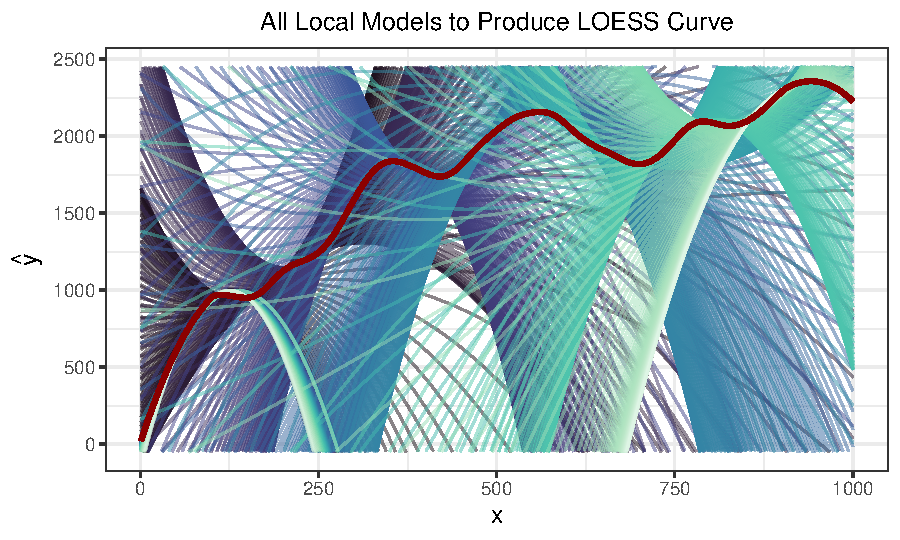
\includegraphics{thesis_files/figure-latex/loess-all-1} 

}

\caption{\label{loess-all}}\label{fig:loess-all}
\end{figure}
Smoothing methods are sensitive to the choice of smoothing parameter \(h\), which represents the fraction of the data that is used for the local polynomial fit.

Methods exist for picking the smoothing parameter \(h\) that minimizes the mean squared error between the predicted values from the estimated line and observed values of the dependent variable, for example, leave-one-out cross-validation or generalized cross-validation.

However, for this work, we used LOESS smoothing to smooth survey data from the COVID-19 Trends and Impact Survey (Reinhart et al., 2021).
We choose the smoothing parameter for each variable based on domain knowledge regarding the level of noise present for each variable of interest. For example, there is substantial noise in the screening test positivity data that reflect trends that do not represent meaningful differences in the screening test positivity. Some trends in the screening sensitivity may be due to scheduled workplace screenings happening at regular time intervals, and some of the variation may be due to the frequency of screening testing due to other variables, such as the access and cost of testing.

Since the ratio \(\frac{\text{screening test positivity}}{\text{overall test positivity}}\) is used to estimate \(\beta = \frac{P(\text{test}_+| S_0, untested)}{P(\text{test}_+|tested)}\), the variability in the screening positivity creates substantial variability in our estimates of \(\beta\).

In light of this variability and the presence of other trends regarding the screening test positivity, we set the span to \(\frac{4}{12} = 0.33\) to fit the local regressions for 4-month intervals with the aim to capture the broader trends over time.

INCLUDE FIGURE OF SMOOTHED ESTIMATES HERE

There was less variabiity in the smoothing span for the weighted percentage of COVID-like Illness, the estimate of \(P(S_1|untested)\). Hence, we set the smoothing parameter to \(0.2\) detect trends at a finer time scale.

Sensitivity analyses with modified versions of the smoothing span of \(\beta\) are included in the appendix in the section INCLUDE SECTION.

\newpage

\hypertarget{kernel-density-estimation}{%
\section{Kernel Density Estimation}\label{kernel-density-estimation}}

\hypertarget{overview-1}{%
\subsection{Overview}\label{overview-1}}

When we have a random sample \(X_1,\dots X_n\) drawn from the density \(f_X\) and we want to estimate \(f_X\) at some set of points, we can use kernel density estimation. This is relevant in this work for estimating \(f^{induced}\).

We define a kernel function as follows (Wasserman, 2006).
\begin{tcolorbox}[title=Definition: Kernel Function]

A kernel function $K$ is a smooth nonnegative function such that 

$$\int K(x) \; dx = 1, \int x K(x) dx = 0, \sigma^2_k \equiv \int x^2 K(x) dx > 0.$$ 
\end{tcolorbox}
The Gaussian kernel \(K(x) = \frac{1}{\sqrt{2\pi}}e^{-x^2/2}\) is commonly used in practice; the tricube kernel, as discussed in the LOESS smoothing section, is another valid kernel function.

The kernel density estimator is

\[\hat f_n(x) = \frac 1n \sum_{i=1}^n \frac 1h K\left(\dfrac{x-X_i}{h} \right)\]

where \(h\) is the smoothing parameter or bandwidth. In Figure \ref{fig:kernel}, we see the effect of increasing the bandwidth \(h\): larger values result in smoother curves, while smaller values result in curves that follow the histogram more closely.
\begin{figure}

{\centering 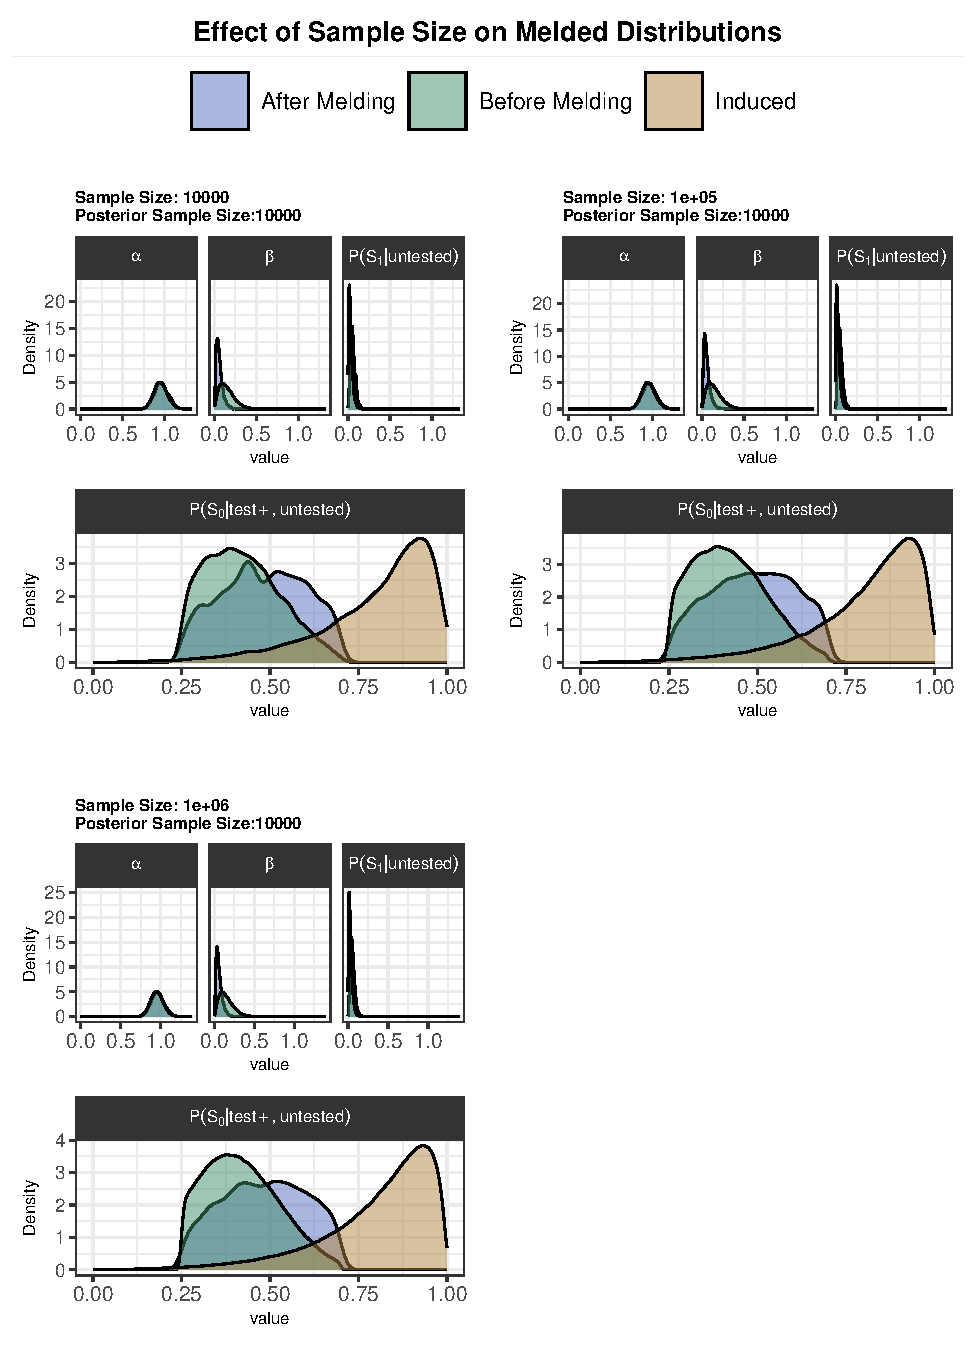
\includegraphics{thesis_files/figure-latex/unnamed-chunk-27-1} 

}

\caption{\label{fig:kernel}}\label{fig:unnamed-chunk-27}
\end{figure}
\hypertarget{bounded-density-estimation}{%
\subsection{Bounded Density Estimation}\label{bounded-density-estimation}}

A question warranting investigation is the choice of kernel given we are working with a bounded variable -- the density we seek to estimate, \(f^{induced}\) is the density of \(P(S_0|\text{untested}, \text{test}_+)\) and hence is bounded between 0 and 1.

One way to handle density estimation for a bounded variable \(X\) is by performing a transformation
\(X=g(Y)\) and then using the change of variables for a probability density to obtain \(f_X(x)\) (Aurelien Pelissier, 2022).

Since \(X \in [0,1]\) and we want to transform it to the range \((-\infty,\infty)\), we can let \(Y = \text{logit}(X) = \log \left( \frac{X}{1-X} \right)\).

We know if we have \(X = g(Y)\), then we can acquire the distribution of \(X\) from that of \(Y\) by considering the change of variables of the probability density functions \(f_X\) and \(f_y\) given by
\[f_X(x) = f_Y(g^{-1}(X)) \;\; \left| \frac{d}{dx} g^{-1}(X) \right|. \tag{1}\]

Thus, in this case, we have \(Y = \text{logit}(X)\), so \(g^{-1}\) is the logit function. By definition of the change of variables formula (1), we have
\[f_X(x) = f_Y(\text{logit}(X)) \;\; \left| \frac{d}{dx} \text{logit}(X) \right|.\]
Computing the derivative and simplifying, we have
\begin{align*} = f_Y(logit(X)) \;\; \left| \frac{d}{dx}log(\frac{x}{1-x}) \right|\\
&= f_Y(logit(X)) \;\; \left| \left(\frac{1-x}{x} \right) (x(1-x)^{-1})' \right|\\ 
&= f_Y(logit(X)) \;\; \left| \left(\frac{1-x}{x} \right) ((1-x)^{-1} + x(1-x)^{-2} ) \right|\\
&= f_Y(logit(X)) \;\; \left| \left(\frac{1-x}{x} \right) \left(\frac{(1-x) + x }{ (1-x)^{2} }\right) \right|\\
&= f_Y(logit(X)) \;\; \left| \left(\frac{1-x}{x} \right) \left(\frac{1 }{ (1-x)^{2} }\right) \right|\\
&= f_Y(logit(X)) \;\; \left|  \frac{1 }{ x (1-x) } \right|.
\end{align*}
This means that we compute \(Y = logit(X)\) and then estimate the density of the unbounded variable \(Y\), and then we can recover the density \(f_X\) by multiplying by \(\frac{1 }{ x (1-x) }\).

In some cases, this approach works well. In Figure \ref{fig:trans}, we simulate a variable \(X \sim Beta(3,2)\) and estimate the density with the transformation approach.
\begin{figure}

{\centering 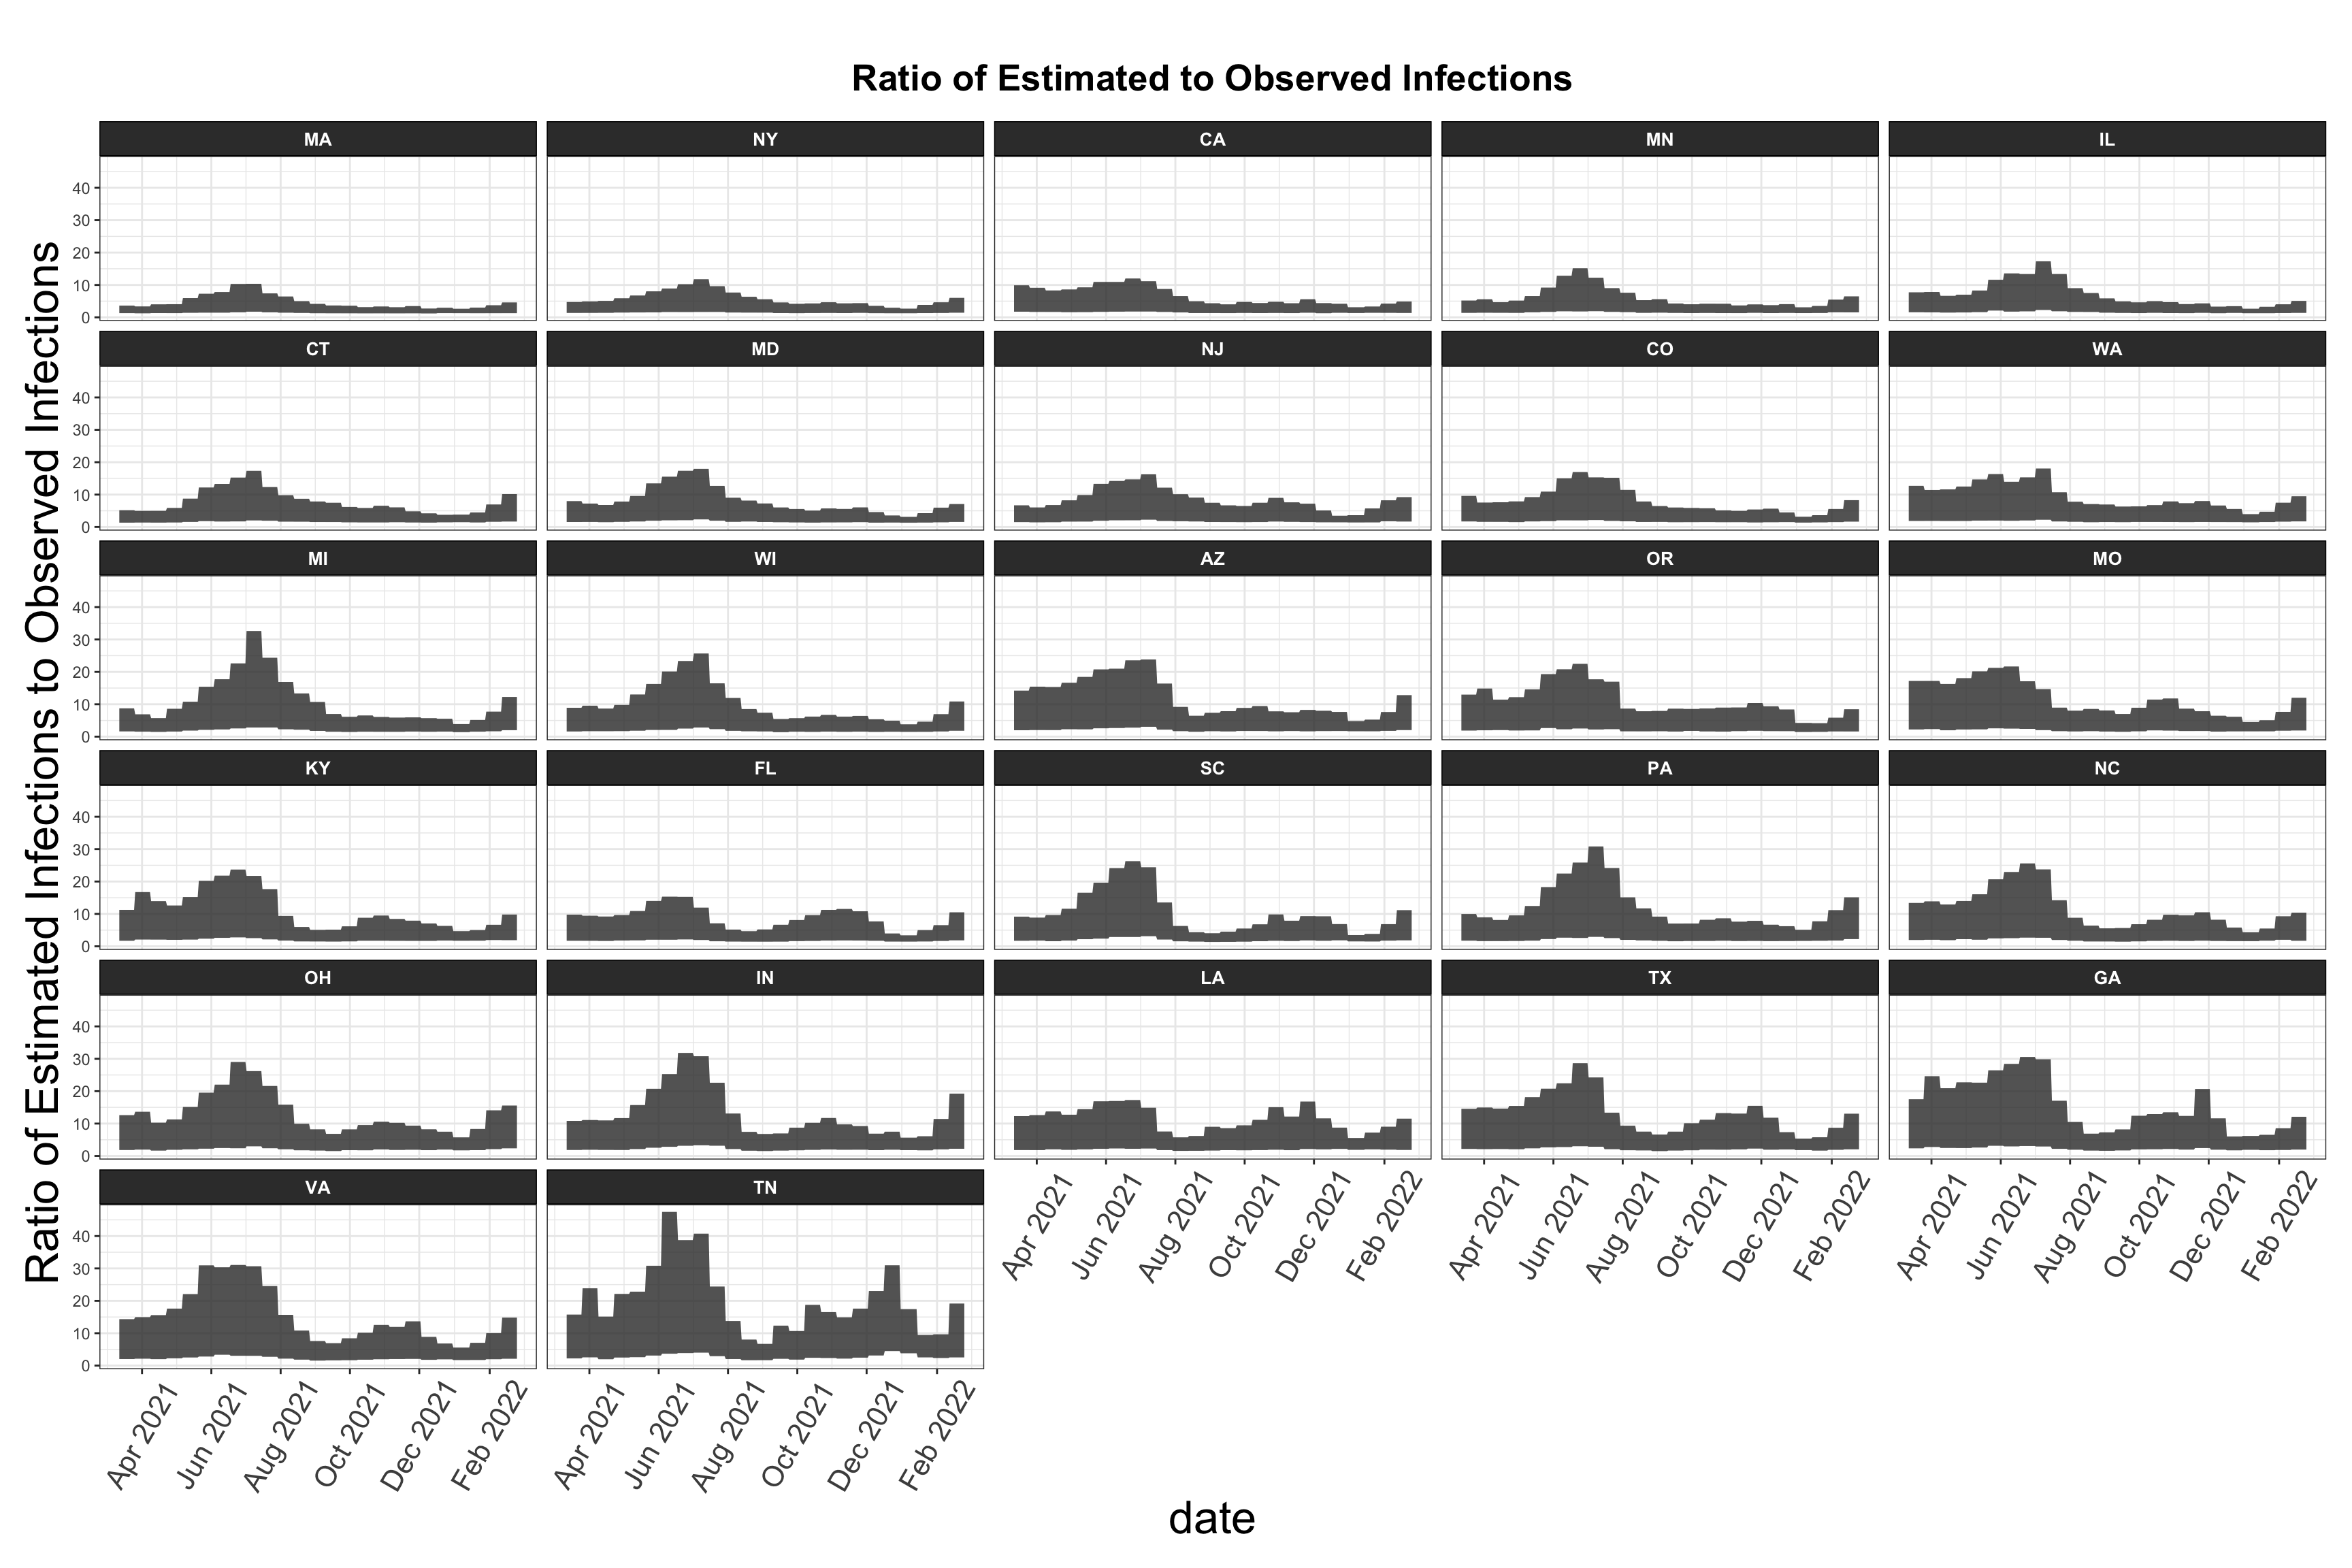
\includegraphics{thesis_files/figure-latex/unnamed-chunk-29-1} 

}

\caption{\label{fig:trans}}\label{fig:unnamed-chunk-29}
\end{figure}
We see the difference between using the transformation approach versus estimating the density of \(X\) without first transforming it to be unbounded in Figure \ref{fig:original}.
\begin{figure}

{\centering 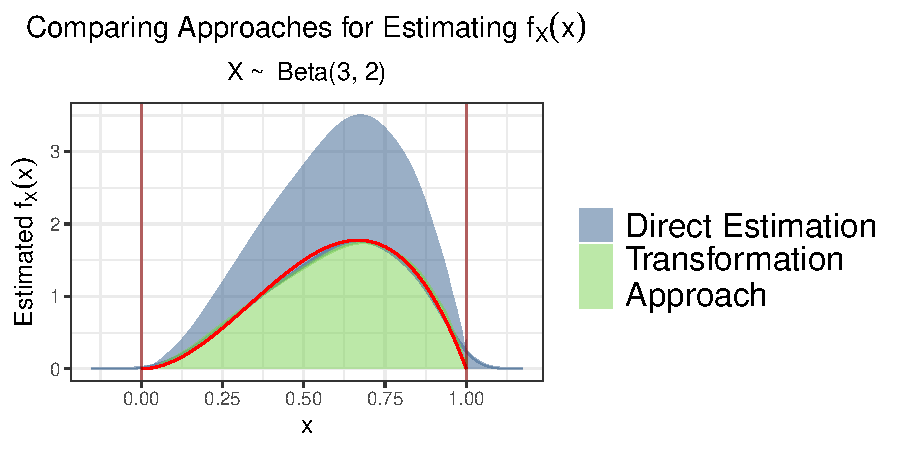
\includegraphics{thesis_files/figure-latex/unnamed-chunk-30-1} 

}

\caption{\label{fig:original}}\label{fig:unnamed-chunk-30}
\end{figure}
However, when we simulate densities that have greater mass toward the boundaries 0 or 1, we see that boundary bias becomes problematic (Figure \ref{fig:compare-beta-params}). This is evident in panels B, C, D, and G of Figure \ref{fig:compare-beta-params}, where the estimated density near the boundaries is a poor estimate of the true density.
\begin{figure}

{\centering 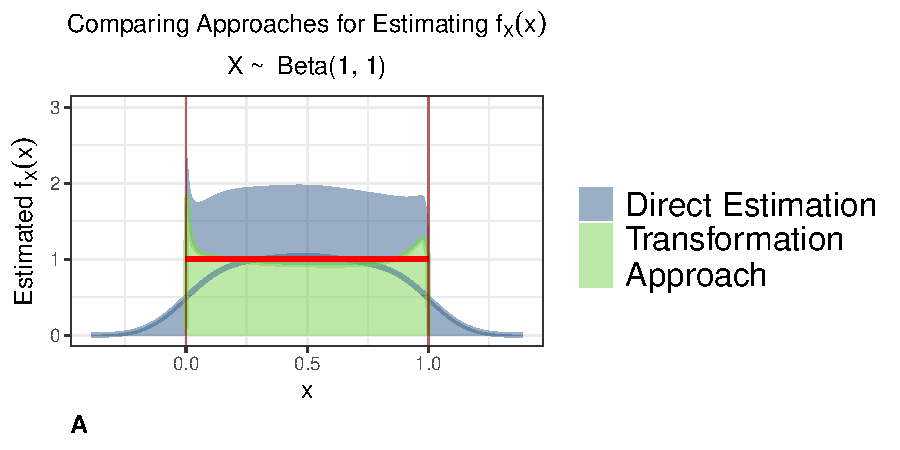
\includegraphics[width=0.49\linewidth]{thesis_files/figure-latex/unnamed-chunk-31-1} 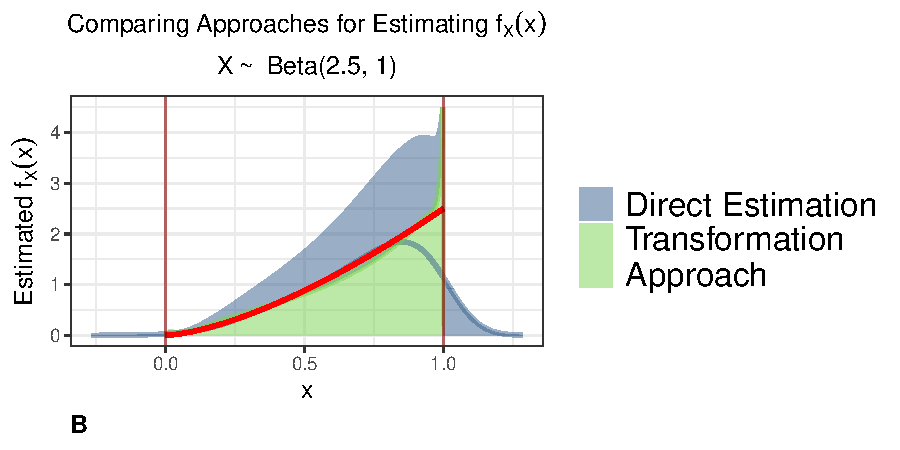
\includegraphics[width=0.49\linewidth]{thesis_files/figure-latex/unnamed-chunk-31-2} 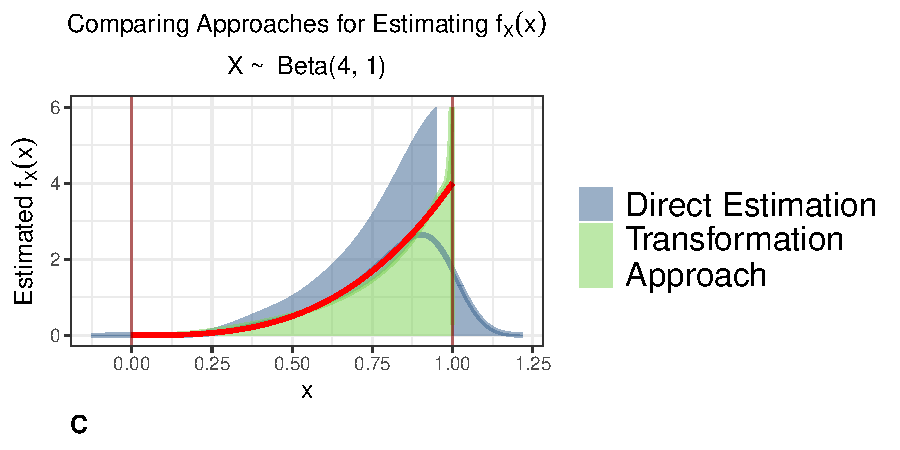
\includegraphics[width=0.49\linewidth]{thesis_files/figure-latex/unnamed-chunk-31-3} 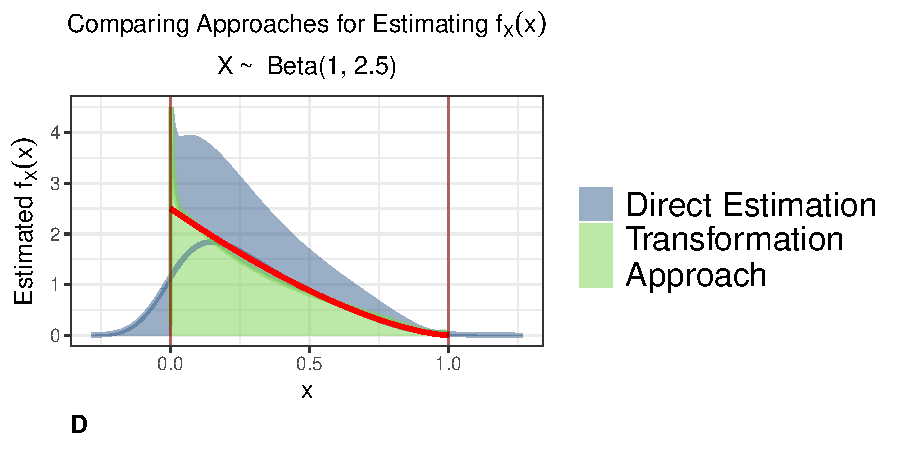
\includegraphics[width=0.49\linewidth]{thesis_files/figure-latex/unnamed-chunk-31-4} 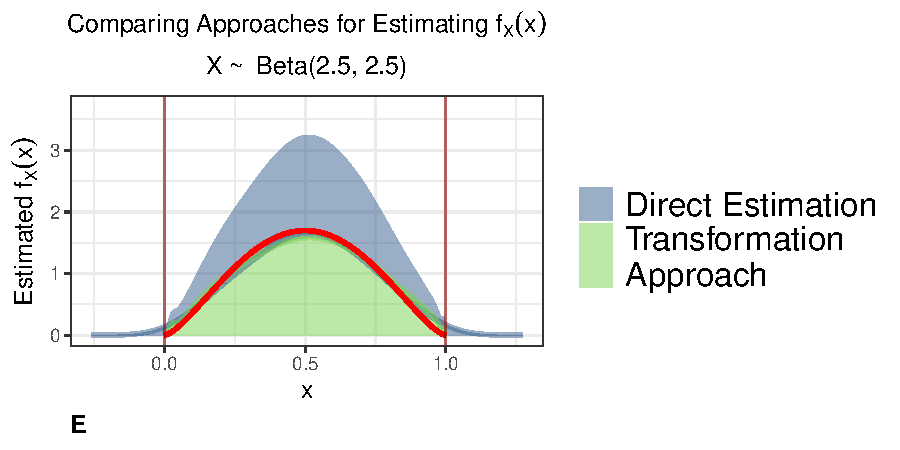
\includegraphics[width=0.49\linewidth]{thesis_files/figure-latex/unnamed-chunk-31-5} 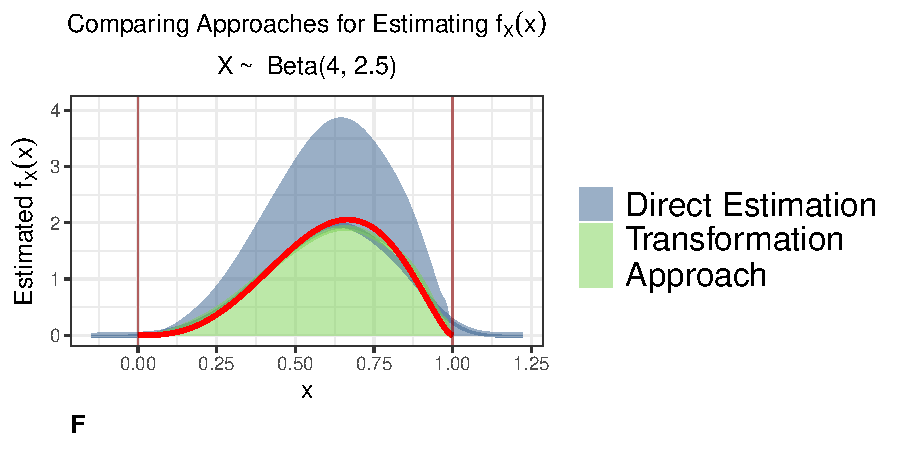
\includegraphics[width=0.49\linewidth]{thesis_files/figure-latex/unnamed-chunk-31-6} 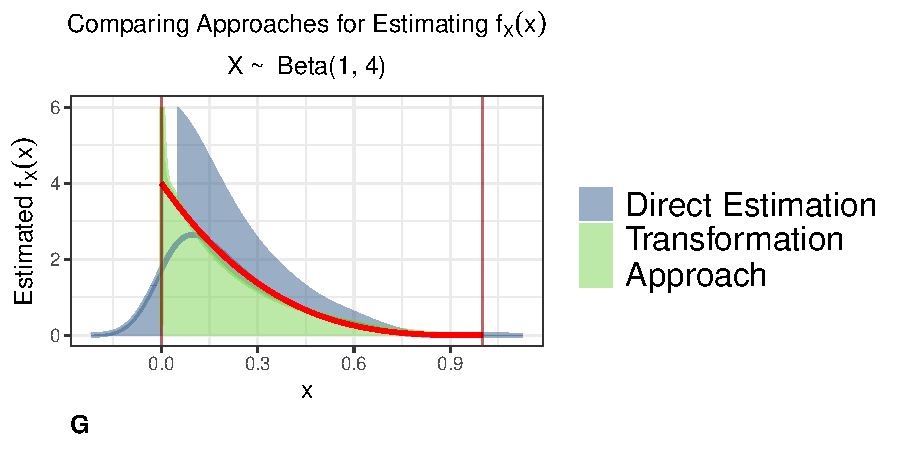
\includegraphics[width=0.49\linewidth]{thesis_files/figure-latex/unnamed-chunk-31-7} 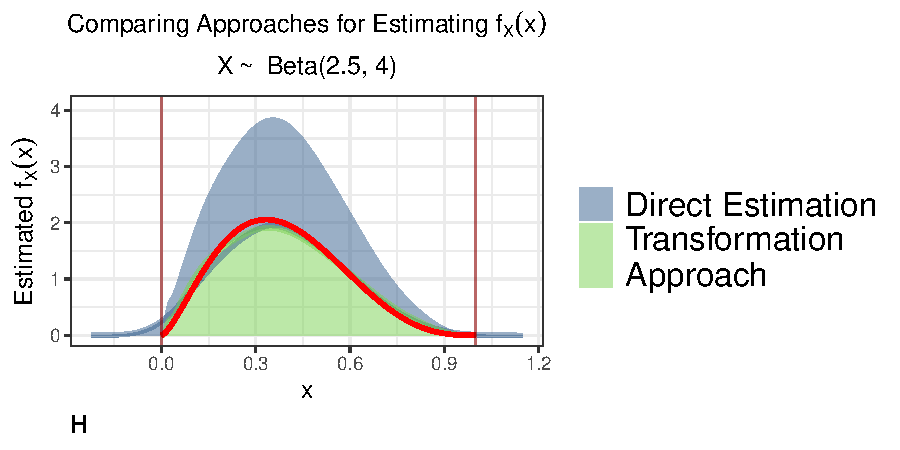
\includegraphics[width=0.49\linewidth]{thesis_files/figure-latex/unnamed-chunk-31-8} 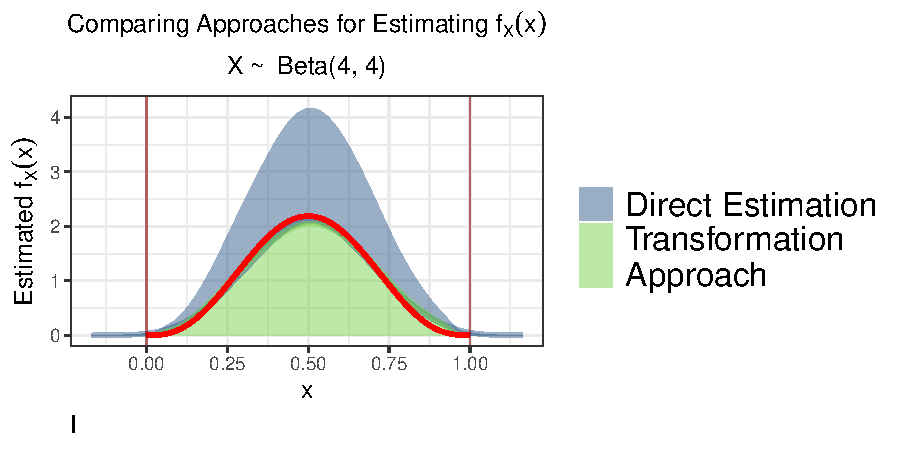
\includegraphics[width=0.49\linewidth]{thesis_files/figure-latex/unnamed-chunk-31-9} 

}

\caption{\label{fig:compare-beta-params}}\label{fig:unnamed-chunk-31}
\end{figure}
An alternative to the transformation approach for density estimation of bounded variables by using beta kernel estimators, which resolves the issue of boundary bias.

As defined in Chen (1999), the most simple beta kernel estimator would be
\[\hat f_1(x) = \dfrac{\sum_{i=1}^n K_{x/b + 1, \; (1-x)/b + 1} (X_i)}{n}\]

where \(K_{\text{shape1}, \text{shape2}}\) is the density function \(Beta(shape1, \; shape2)\).

However, Chen (1999) show that the modified beta kernel estimator \(\hat f_2(x)\) has lower variance and bias than \(\hat f_1\), where we define \(\hat f_2\) as follows:

\[
\hat f_2(x)  = \dfrac{\sum_{i=1}^n K_{x,b}^*(X_i)}{n},\]

\[K^*_{x,b} = \begin{cases}K_{x/b, \; (1-x)/b }(t)  & \text{if }x \in [2b,1-2b] \\
K_{\rho(x), \; (1-x)/b } (t)  & \text{if } x \in [0,2b) \\
K_{x/b, \; \rho(1-x)}(t) & \text{if } x\in(1-2b,1]
\end{cases},
\]
\[\rho(x,b) = 2b^2 + 2.5 - \sqrt{b^2 + 6b^2 +2.25-x^2 -x/b}.\]

Notably, for beta kernel estimators, the shape of the kernel depends on \(x\) (Figure \ref{fig:depends-on-x}).
\begin{figure}

{\centering 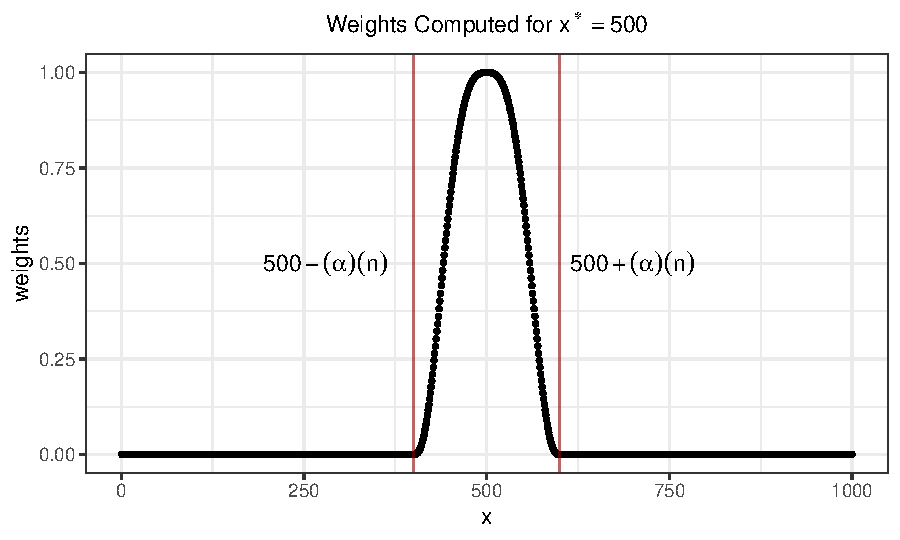
\includegraphics{thesis_files/figure-latex/unnamed-chunk-33-1} 

}

\caption{\label{fig:depends-on-x}}\label{fig:unnamed-chunk-33}
\end{figure}
As we did in Figure \ref{fig:compare-beta-params}, we can compare the performance of the beta kernel \(\hat f_2\) for estimating the density of samples from different beta distributions (Figure \ref{fig:comp-beta}).
\begin{figure}

{\centering 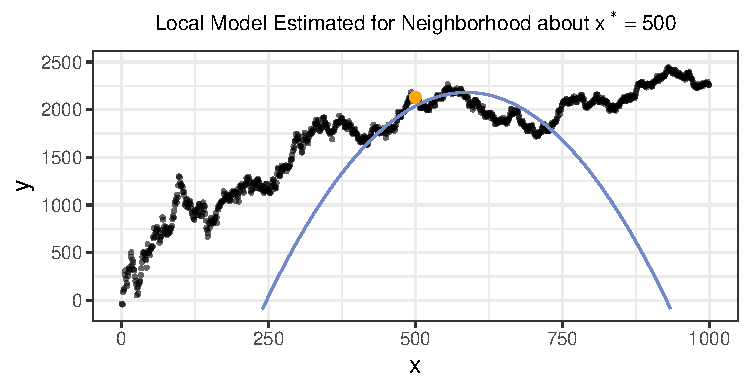
\includegraphics[width=0.48\linewidth]{thesis_files/figure-latex/unnamed-chunk-34-1} 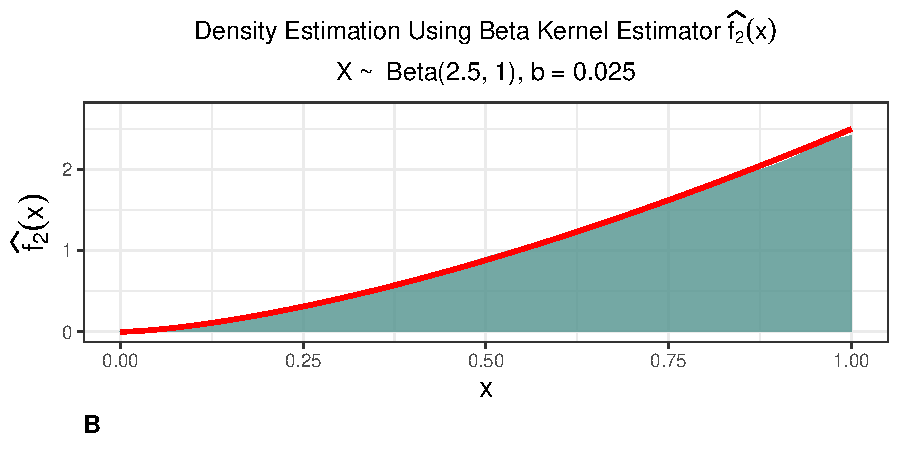
\includegraphics[width=0.48\linewidth]{thesis_files/figure-latex/unnamed-chunk-34-2} 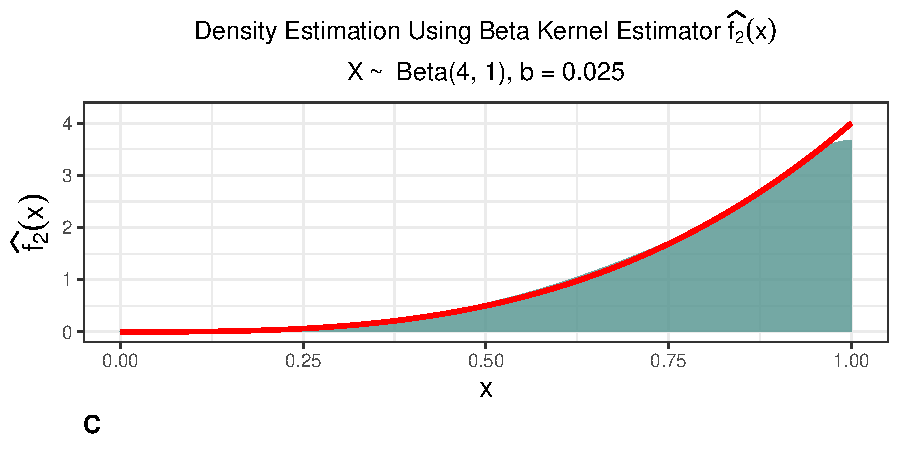
\includegraphics[width=0.48\linewidth]{thesis_files/figure-latex/unnamed-chunk-34-3} 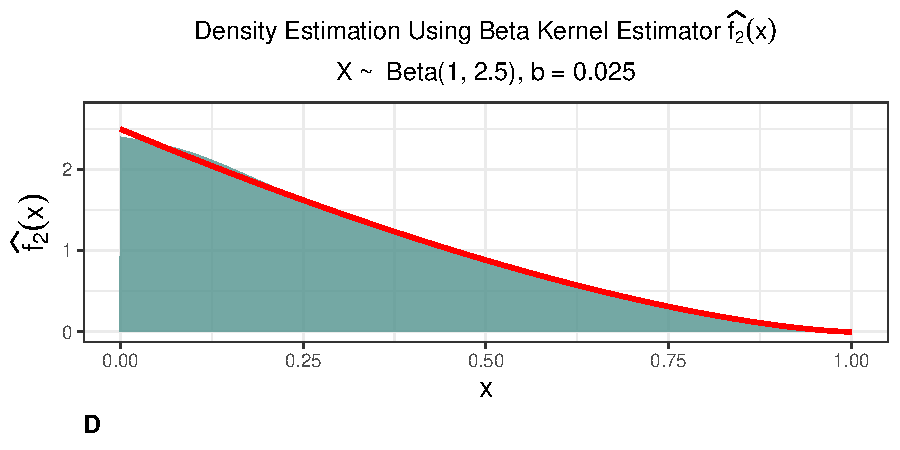
\includegraphics[width=0.48\linewidth]{thesis_files/figure-latex/unnamed-chunk-34-4} 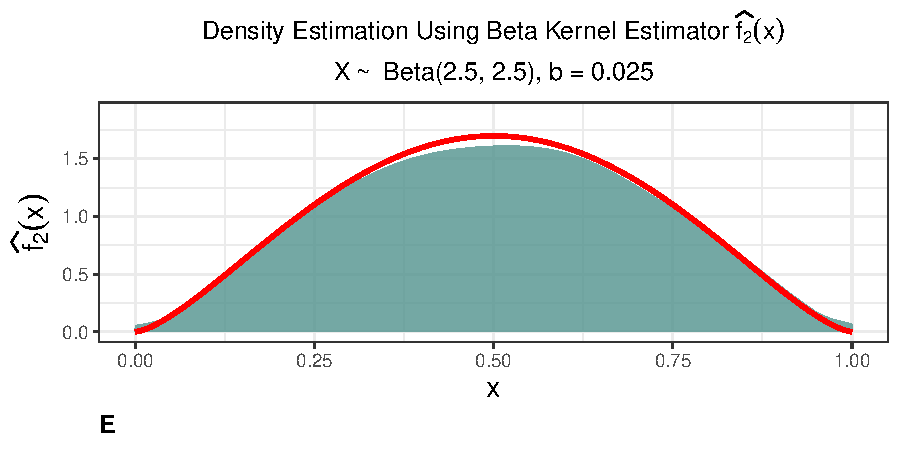
\includegraphics[width=0.48\linewidth]{thesis_files/figure-latex/unnamed-chunk-34-5} 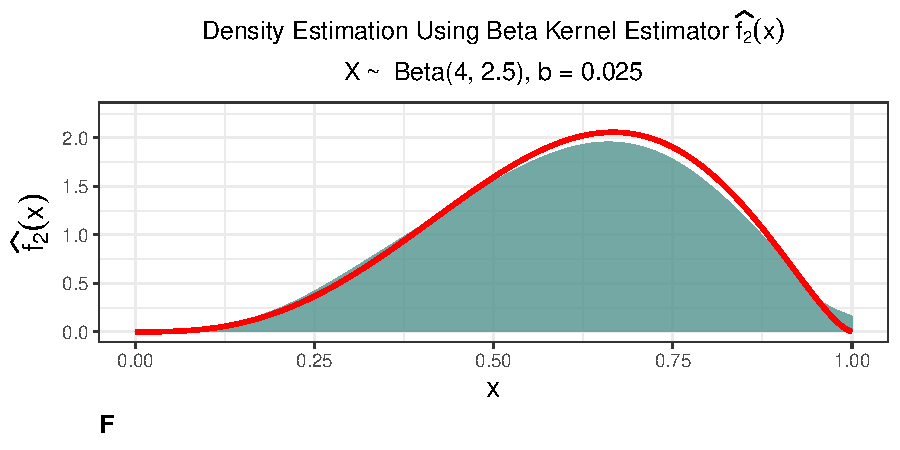
\includegraphics[width=0.48\linewidth]{thesis_files/figure-latex/unnamed-chunk-34-6} 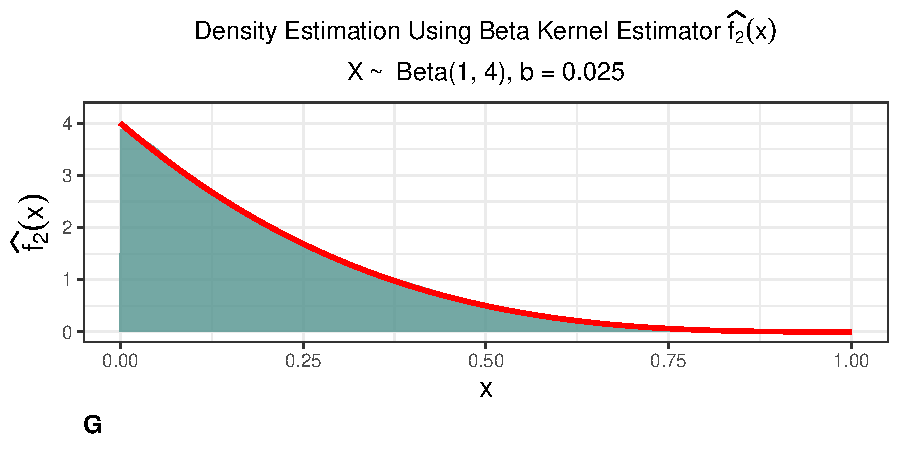
\includegraphics[width=0.48\linewidth]{thesis_files/figure-latex/unnamed-chunk-34-7} 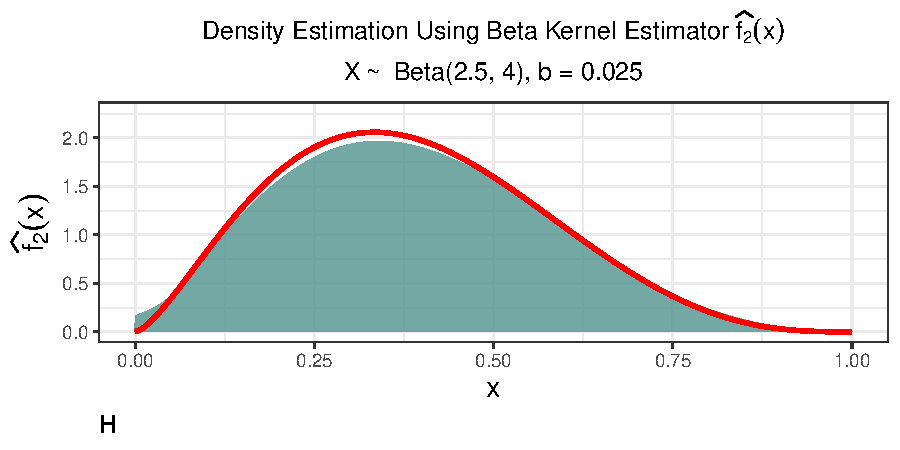
\includegraphics[width=0.48\linewidth]{thesis_files/figure-latex/unnamed-chunk-34-8} 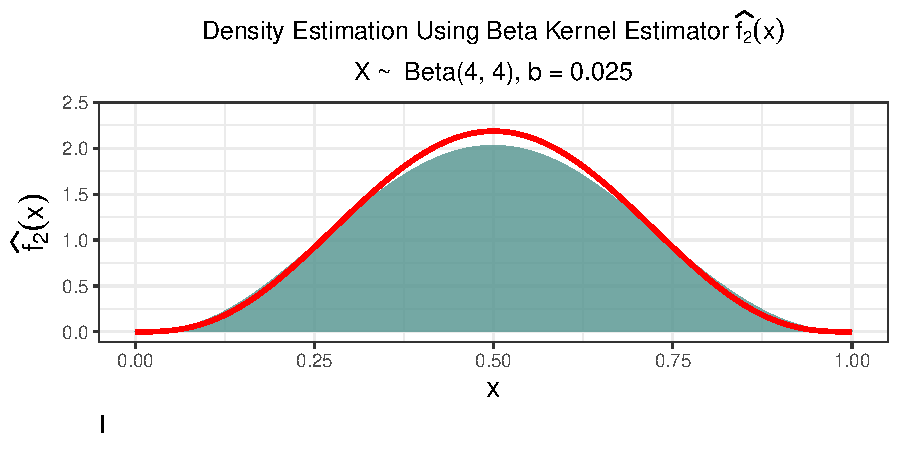
\includegraphics[width=0.48\linewidth]{thesis_files/figure-latex/unnamed-chunk-34-9} 

}

\caption{\label{fig:comp-beta}}\label{fig:unnamed-chunk-34}
\end{figure}
\hypertarget{definition-of-prior-distributions-for-bias-parameters}{%
\chapter{Definition of Prior Distributions for Bias Parameters}\label{definition-of-prior-distributions-for-bias-parameters}}

Placeholder

\hypertarget{background-on-the-beta-distribution}{%
\section{Background on the Beta Distribution}\label{background-on-the-beta-distribution}}

\hypertarget{background-on-the-gamma-distribution}{%
\section{Background on the Gamma Distribution}\label{background-on-the-gamma-distribution}}

\hypertarget{definition-of-prior-distributions-for-incomplete-testing-correction}{%
\section{Definition of Prior Distributions for Incomplete Testing Correction}\label{definition-of-prior-distributions-for-incomplete-testing-correction}}

\hypertarget{defining-ps_1untested}{%
\subsection{\texorpdfstring{Defining \(P(S_1|Untested)\)}{Defining P(S\_1\textbar Untested)}}\label{defining-ps_1untested}}

\hypertarget{defining-alpha}{%
\subsection{\texorpdfstring{Defining \(\alpha\)}{Defining \textbackslash alpha}}\label{defining-alpha}}

\hypertarget{defining-beta}{%
\subsection{\texorpdfstring{Defining \(\beta\)}{Defining \textbackslash beta}}\label{defining-beta}}

\hypertarget{defining-ps_0testuntested}{%
\subsection{\texorpdfstring{Defining \(P(S_0|test+,untested)\)}{Defining P(S\_0\textbar test+,untested)}}\label{defining-ps_0testuntested}}

\hypertarget{definition-of-priors-for-test-inaccuracy-correction}{%
\section{Definition of Priors for Test Inaccuracy Correction}\label{definition-of-priors-for-test-inaccuracy-correction}}

\hypertarget{defining-test-sensitivity-s_e}{%
\subsection{\texorpdfstring{Defining Test Sensitivity (\(S_e\))}{Defining Test Sensitivity (S\_e)}}\label{defining-test-sensitivity-s_e}}

\hypertarget{defining-test-specificity-s_p}{%
\section{\texorpdfstring{Defining Test Specificity (\(S_p\))}{Defining Test Specificity (S\_p)}}\label{defining-test-specificity-s_p}}

\hypertarget{summary-table-of-bias-parameter-distributions}{%
\section{Summary Table of Bias Parameter Distributions}\label{summary-table-of-bias-parameter-distributions}}

\hypertarget{correction-for-incomplete-testing}{%
\section{Correction for Incomplete Testing}\label{correction-for-incomplete-testing}}

\hypertarget{correction-for-diagnostic-test-inaccuracy}{%
\section{Correction for Diagnostic Test Inaccuracy}\label{correction-for-diagnostic-test-inaccuracy}}

\hypertarget{derivation-of-formula-for-correction-for-diagnostic-test-inaccuracy}{%
\subsection{Derivation of Formula for Correction for Diagnostic Test Inaccuracy}\label{derivation-of-formula-for-correction-for-diagnostic-test-inaccuracy}}

\hypertarget{details-of-implementation}{%
\chapter{Details of Implementation}\label{details-of-implementation}}
\begin{itemize}
\tightlist
\item
  Describe each step here
\item
  Mention reproducible workflow with make
\end{itemize}
\hypertarget{reproducible-workflow}{%
\section{Reproducible Workflow}\label{reproducible-workflow}}

\hypertarget{results}{%
\chapter{Results}\label{results}}

Placeholder

\hypertarget{county-level}{%
\section{County-level}\label{county-level}}

\hypertarget{state-level}{%
\section{State-level}\label{state-level}}

\hypertarget{comparison-to-the-covidestim-model}{%
\section{Comparison to the Covidestim Model}\label{comparison-to-the-covidestim-model}}

\hypertarget{overview-2}{%
\subsection{Overview}\label{overview-2}}

\hypertarget{the-covidestim-model}{%
\subsection{The Covidestim Model}\label{the-covidestim-model}}

\hypertarget{assumptions}{%
\subsection{Assumptions}\label{assumptions}}

\hypertarget{comparison-to-other-indicators}{%
\section{Comparison to Other Indicators}\label{comparison-to-other-indicators}}

\hypertarget{limitations-of-this-comparison}{%
\section{Limitations of this Comparison}\label{limitations-of-this-comparison}}

\hypertarget{simulation-bivariate-normal}{%
\subsection{Simulation: Bivariate Normal}\label{simulation-bivariate-normal}}

\hypertarget{derivation-of-the-distribution-of-xy-for-bivariate-normal}{%
\subsection{Derivation of the Distribution of X+Y for Bivariate Normal}\label{derivation-of-the-distribution-of-xy-for-bivariate-normal}}

\hypertarget{seropositivity-data}{%
\section{Seropositivity Data}\label{seropositivity-data}}

\hypertarget{county-level-1}{%
\section{County-level}\label{county-level-1}}

\hypertarget{state-level-1}{%
\section{State-level}\label{state-level-1}}

\hypertarget{appendix}{%
\chapter{Appendix}\label{appendix}}

Placeholder

\hypertarget{smoothing-span}{%
\section{Smoothing Span}\label{smoothing-span}}

\hypertarget{changing-span-for-loess-smoothing-of-beta}{%
\subsection{\texorpdfstring{Changing SPAN for LOESS Smoothing of \(\beta\)}{Changing SPAN for LOESS Smoothing of \textbackslash beta}}\label{changing-span-for-loess-smoothing-of-beta}}

\hypertarget{changing-mean-and-variance-for-prior-distribution-specifications}{%
\section{Changing Mean and Variance for Prior Distribution Specifications}\label{changing-mean-and-variance-for-prior-distribution-specifications}}

\hypertarget{references}{%
\chapter*{References}\label{references}}
\addcontentsline{toc}{chapter}{References}

Placeholder

\hypertarget{refs}{}
\begin{CSLReferences}{1}{0}
\leavevmode\vadjust pre{\hypertarget{ref-aurelienpelissier2022}{}}%
Aurelien Pelissier. (2022, February 4). Density Estimation for Bounded Variables. Retrieved March 19, 2023, from \url{https://medium.com/mlearning-ai/density-estimation-for-bounded-variables-7d68f633e772}

\leavevmode\vadjust pre{\hypertarget{ref-blitzsteinIntroductionProbability2019}{}}%
Blitzstein, J. K., \& Hwang, J. (2019). \emph{Introduction to probability} (Second edition). Boca Raton: CRC Press.

\leavevmode\vadjust pre{\hypertarget{ref-carvalho2023}{}}%
Carvalho, L. M., Villela, D. A. M., Coelho, F. C., \& Bastos, L. S. (2023). Bayesian Inference for the Weights in Logarithmic Pooling. \emph{Bayesian Analysis}, \emph{18}(1). http://doi.org/\href{https://doi.org/10.1214/22-BA1311}{10.1214/22-BA1311}

\leavevmode\vadjust pre{\hypertarget{ref-chambers1997}{}}%
Chambers, J. M. (Ed.). (1997). \emph{Statistical models in S} (Reprint). London: Chapman \& Hall.

\leavevmode\vadjust pre{\hypertarget{ref-chen1999}{}}%
Chen, S. X. (1999). Beta kernel estimators for density functions. \emph{Computational Statistics \& Data Analysis}, \emph{31}(2), 131--145. http://doi.org/\href{https://doi.org/10.1016/S0167-9473(99)00010-9}{10.1016/S0167-9473(99)00010-9}

\leavevmode\vadjust pre{\hypertarget{ref-genest1986}{}}%
Genest, C., McConway, K. J., \& Schervish, M. J. (1986). Characterization of Externally Bayesian Pooling Operators. \emph{The Annals of Statistics}, \emph{14}(2), 487--501. Retrieved from \url{https://www.jstor.org/stable/2241231}

\leavevmode\vadjust pre{\hypertarget{ref-greenland2016}{}}%
Greenland, S., Senn, S. J., Rothman, K. J., Carlin, J. B., Poole, C., Goodman, S. N., \& Altman, D. G. (2016). Statistical tests, P values, confidence intervals, and power: a guide to misinterpretations. \emph{European Journal of Epidemiology}, \emph{31}(4), 337--350. http://doi.org/\href{https://doi.org/10.1007/s10654-016-0149-3}{10.1007/s10654-016-0149-3}

\leavevmode\vadjust pre{\hypertarget{ref-lash2009}{}}%
Lash, T. L., Fox, M. P., \& Fink, A. K. (2009). \emph{Applying Quantitative Bias Analysis to Epidemiologic Data}. New York, NY: Springer New York. http://doi.org/\href{https://doi.org/10.1007/978-0-387-87959-8}{10.1007/978-0-387-87959-8}

\leavevmode\vadjust pre{\hypertarget{ref-ma2021}{}}%
Ma, Q., Liu, J., Liu, Q., Kang, L., Liu, R., Jing, W., \ldots{} Liu, M. (2021). Global Percentage of Asymptomatic SARS-CoV-2 Infections Among the Tested Population and Individuals With Confirmed COVID-19 Diagnosis: A Systematic Review and Meta-analysis. \emph{JAMA Network Open}, \emph{4}(12), e2137257. http://doi.org/\href{https://doi.org/10.1001/jamanetworkopen.2021.37257}{10.1001/jamanetworkopen.2021.37257}

\leavevmode\vadjust pre{\hypertarget{ref-neyman1937}{}}%
Neyman, J. (1937). Outline of a Theory of Statistical Estimation Based on the Classical Theory of Probability. \emph{Philosophical Transactions of the Royal Society of London. Series A, Mathematical and Physical Sciences}, \emph{236}(767), 333--380. http://doi.org/\href{https://doi.org/10.1098/rsta.1937.0005}{10.1098/rsta.1937.0005}

\leavevmode\vadjust pre{\hypertarget{ref-petersen2021}{}}%
Petersen, J. M., Ranker, L. R., Barnard-Mayers, R., MacLehose, R. F., \& Fox, M. P. (2021). A systematic review of quantitative bias analysis applied to epidemiological research. \emph{International Journal of Epidemiology}, \emph{50}(5), 1708--1730. http://doi.org/\href{https://doi.org/10.1093/ije/dyab061}{10.1093/ije/dyab061}

\leavevmode\vadjust pre{\hypertarget{ref-poole2000}{}}%
Poole, D., \& Raftery, A. E. (2000). Inference for Deterministic Simulation Models: The Bayesian Melding Approach. \emph{Journal of the American Statistical Association}, \emph{95}(452), 1244--1255. http://doi.org/\href{https://doi.org/10.1080/01621459.2000.10474324}{10.1080/01621459.2000.10474324}

\leavevmode\vadjust pre{\hypertarget{ref-powers2011}{}}%
Powers, K. A., Ghani, A. C., Miller, W. C., Hoffman, I. F., Pettifor, A. E., Kamanga, G., \ldots{} Cohen, M. S. (2011). The role of acute and early HIV infection in the spread of HIV and implications for transmission prevention strategies in Lilongwe, Malawi: a modelling study. \emph{The Lancet}, \emph{378}(9787), 256--268. http://doi.org/\href{https://doi.org/10.1016/S0140-6736(11)60842-8}{10.1016/S0140-6736(11)60842-8}

\leavevmode\vadjust pre{\hypertarget{ref-reinhart2021}{}}%
Reinhart, A., Brooks, L., Jahja, M., Rumack, A., Tang, J., Agrawal, S., \ldots{} Tibshirani, R. J. (2021). An open repository of real-time COVID-19 indicators. \emph{Proceedings of the National Academy of Sciences}, \emph{118}(51), e2111452118. http://doi.org/\href{https://doi.org/10.1073/pnas.2111452118}{10.1073/pnas.2111452118}

\leavevmode\vadjust pre{\hypertarget{ref-robson2014}{}}%
Robson, B. J. (2014). When do aquatic systems models provide useful predictions, what is changing, and what is next? \emph{Environmental Modelling \& Software}, \emph{61}, 287--296. http://doi.org/\href{https://doi.org/10.1016/j.envsoft.2014.01.009}{10.1016/j.envsoft.2014.01.009}

\leavevmode\vadjust pre{\hypertarget{ref-rubin1987}{}}%
Rubin, D. B. (1987). The Calculation of Posterior Distributions by Data Augmentation: Comment: A Noniterative Sampling/Importance Resampling Alternative to the Data Augmentation Algorithm for Creating a Few Imputations When Fractions of Missing Information Are Modest: The SIR Algorithm. \emph{Journal of the American Statistical Association}, \emph{82}(398), 543. http://doi.org/\href{https://doi.org/10.2307/2289460}{10.2307/2289460}

\leavevmode\vadjust pre{\hypertarget{ref-rubin2004}{}}%
Rubin, D. B., Gelman, A., \& Meng, X.-L. (Eds.). (2004). \emph{Applied Bayesian modeling and causal inference from incomplete-data perspectives: an essential journey with Donald Rubin's statistical family}. Chichester, West Sussex, England\,; Hoboken, NJ: Wiley.

\leavevmode\vadjust pre{\hypertarget{ref-sah2021}{}}%
Sah, P., Fitzpatrick, M. C., Zimmer, C. F., Abdollahi, E., Juden-Kelly, L., Moghadas, S. M., \ldots{} Galvani, A. P. (2021). Asymptomatic SARS-CoV-2 infection: A systematic review and meta-analysis. \emph{Proceedings of the National Academy of Sciences}, \emph{118}(34), e2109229118. http://doi.org/\href{https://doi.org/10.1073/pnas.2109229118}{10.1073/pnas.2109229118}

\leavevmode\vadjust pre{\hypertarget{ref-sevcikova2007}{}}%
Ševčíková, H., Raftery, A. E., \& Waddell, P. A. (2007). Assessing uncertainty in urban simulations using Bayesian melding. \emph{Transportation Research Part B: Methodological}, \emph{41}(6), 652--669. http://doi.org/\href{https://doi.org/10.1016/j.trb.2006.11.001}{10.1016/j.trb.2006.11.001}

\leavevmode\vadjust pre{\hypertarget{ref-wasserman2006}{}}%
Wasserman, L. (2006). \emph{All of nonparametric statistics}. New York: Springer.

\end{CSLReferences}

% Index?

\end{document}
